% !TEX program = xelatex
% !TEX encoding = UTF-8
\documentclass[11pt,a4paper]{article}
\usepackage[a4paper,top=2.4cm,bottom=2.4cm,left=2.3cm,right=2.3cm]{geometry}
\usepackage{fontspec}
% Шрифты TeX Live (есть в Overleaf): CMU Serif и CMU Typewriter — Computer Modern с кириллицей; математика — Latin Modern Math.
\setmainfont{cmunrm}[Extension=.otf,UprightFont=*,BoldFont=cmunbx,ItalicFont=cmunti,BoldItalicFont=cmunbi]
\setmonofont{cmuntt}[Extension=.otf,UprightFont=*,BoldFont=cmuntb,ItalicFont=cmunit,BoldItalicFont=cmuntx,Scale=0.95]
\usepackage{unicode-math}
\setmathfont{latinmodern-math.otf}
\usepackage[english,main=russian]{babel}
\usepackage{newunicodechar}
\newunicodechar{≤}{\ensuremath{\leq}}\newunicodechar{≥}{\ensuremath{\geq}}\newunicodechar{≈}{\ensuremath{\approx}}
\newunicodechar{→}{\ensuremath{\rightarrow}}\newunicodechar{↑}{\ensuremath{\uparrow}}\newunicodechar{↓}{\ensuremath{\downarrow}}
\newunicodechar{σ}{\ensuremath{\sigma}}\newunicodechar{λ}{\ensuremath{\lambda}}\newunicodechar{ρ}{\ensuremath{\rho}}\newunicodechar{ξ}{\ensuremath{\xi}}\newunicodechar{τ}{\ensuremath{\tau}}\newunicodechar{ω}{\ensuremath{\omega}}\newunicodechar{ζ}{\ensuremath{\zeta}}\newunicodechar{ε}{\ensuremath{\varepsilon}}
\newunicodechar{×}{\ensuremath{\times}}\newunicodechar{−}{\ensuremath{-}}
\usepackage{xcolor}
\definecolor{ink}{HTML}{111111}
\definecolor{accent}{HTML}{14602B}
\definecolor{rule}{HTML}{9AA39D}
\definecolor{boxbg}{HTML}{F2F4F2}
\usepackage{amsmath}
\usepackage{graphicx}
\usepackage{float}
\usepackage{caption}
\captionsetup{font=small,labelfont=bf,justification=centering,singlelinecheck=false,skip=6pt}
\usepackage{longtable,booktabs,array}
\usepackage{calc}
\usepackage{etoolbox}
\makeatletter
\patchcmd\longtable{\par}{\if@noskipsec\mbox{}\fi\par}{}{}
\makeatother
\usepackage{footnotehyper}
\makesavenoteenv{longtable}
\newcounter{none}\def\LTcaptype{none}
\setlength{\LTpre}{8pt}\setlength{\LTpost}{10pt}
\renewcommand{\arraystretch}{1.18}
\usepackage{enumitem}
\setlist{nosep,leftmargin=1.6em,topsep=3pt}
\setlist[enumerate]{label=\arabic*.}
\usepackage{fancyvrb}
\usepackage{fvextra}
\DefineVerbatimEnvironment{verbatim}{Verbatim}{fontsize=\scriptsize,breaklines=true,breakanywhere=true,frame=single,framesep=3mm,rulecolor=\color{rule},formatcom=\color{ink}}
\usepackage{titlesec}
\titleformat{\section}{\Large\bfseries\color{ink}}{\thesection.}{0.6em}{}[{\color{rule}\titlerule}]
\titleformat{name=\section,numberless}{\Large\bfseries\color{ink}}{}{0em}{}[{\color{rule}\titlerule}]
\titleformat{\subsection}{\large\bfseries\color{ink}}{\thesubsection.}{0.6em}{}
\titlespacing*{\section}{0pt}{2.2em}{0.9em}
\titlespacing*{\subsection}{0pt}{1.5em}{0.5em}
\usepackage{needspace}
\pretocmd{\section}{\Needspace*{12\baselineskip}}{}{}
\pretocmd{\subsection}{\Needspace*{5\baselineskip}}{}{}
\usepackage{fancyhdr}
\pagestyle{fancy}\fancyhf{}
\fancyhead[L]{\small\itshape Типы муниципальных экономик России}
\fancyhead[R]{\small Ахрамешин А.\,С., Маркелов В.\,Л.}
\fancyfoot[C]{\small\thepage}
\renewcommand{\headrulewidth}{0.3pt}
\usepackage[hidelinks,unicode,pdftitle={Типы муниципальных экономик России: динамическая кластеризация на атрибутированной сети},pdfauthor={Ахрамешин А. С., Маркелов В. Л.}]{hyperref}
\usepackage{xurl}
\urlstyle{same}
\providecommand{\tightlist}{\setlength{\itemsep}{1pt}\setlength{\parskip}{0pt}}
\setlength{\parindent}{1.4em}\setlength{\parskip}{0pt}
\linespread{1.07}
\emergencystretch=2em
\sloppy
\newenvironment{absbox}{\par\begingroup\small\setlength{\parindent}{0pt}\leftskip=1.2em\rightskip=1.2em\ignorespaces}{\par\endgroup}
\begin{document}
\thispagestyle{plain}
\begin{center}
{\LARGE\bfseries\color{ink} Типология муниципальных экономик России: динамическая кластеризация на атрибутированной сети с годовыми окнами\par}
\vspace{1.1em}
{\large Ахрамешин А. С., Маркелов В. Л.\par}
\vspace{0.5em}
{\small\itshape Онлайн-конкурс СберИндекса 2026, направление «Кластеризация». Октябрь 2026.\par}
\end{center}
\vspace{0.8em}
{\color{rule}\hrule}
\vspace{0.9em}
\begin{absbox}
\textbf{Аннотация.} Работа посвящена типологии 1~776 российских муниципальных образований (МО) по структуре безналичных расходов жителей и экономическому контексту на 13 скользящих годовых окнах (декабрь 2023 --- декабрь 2024). МО образуют динамическую атрибутированную сеть: вершины описываются семью признаками расходов (логарифм уровня и шесть композиционных координат) и девятью признаками контекста по данным Росстата, рёбра задаются косинусным сходством годовых профилей расходов. Предложен метод GS-TKM (graph-smoothed temporal k-means): однократное сглаживание признаков по графу сходства, единые для всех окон центры типов и точная условная траектория типов каждой территории по алгоритму Витерби со штрафом за смену типа. По протоколу выбора выделено 5 типов; согласие разбиений при 50 пересборках на подвыборках (ARI) составляет 0,893. Типы различаются по показателям, не входившим в разбиение: региональный интервал эффекта типа целиком выше нуля для 5 из 6 внешних показателей Росстата и СберИндекса, а после контроля населения и зарплаты --- для 3 из 6. Тип не улучшает пространственный перенос прогноза роста расходов сверх непрерывных признаков (снижение MAE 0,0001 лог. пункта; интервал включает нуль). Часть смен типа за год отражает общий сдвиг потребления по стране: после центрирования признаков по окнам доля сменивших тип снижается с 16,9\% до 7,8\%. Результаты воспроизводимы, включая пересборки, чувствительность и проверки; приведены также ограничения метода.
\end{absbox}
\vspace{0.7em}
{\color{rule}\hrule}
\vspace{0.4em}
\section{Введение}\label{ux432ux432ux435ux434ux435ux43dux438ux435}

\subsection{Постановка задачи}\label{ux43fux43eux441ux442ux430ux43dux43eux432ux43aux430-ux437ux430ux434ux430ux447ux438}

Требуется построить типологию муниципальных образований (МО) на динамической атрибутированной сети: вершины --- МО (или объединённая территория), атрибуты --- структура расходов и экономический контекст, рёбра --- сходство профилей расходов; атрибуты и рёбра пересчитываются для каждого из 13 окон. Типы должны быть согласованы и по атрибутам, и по связям, а переходы территорий между типами --- описаны.

Задача содержит две методологические трудности. Во-первых, у понятия «сходство» нет единственного операционального определения: сходство структуры трат, совместное движение рядов, сдвиг рядов друг относительно друга и географическая близость задают разные отношения между территориями (раздел 4). Во-вторых, при отсутствии эталонной разметки качество кластеризации нельзя измерить напрямую. Оно оценивается внутренними индексами (раздел 6), устойчивостью к выбору подвыборки и инициализации (раздел 9), показателями, не входившими в разбиение (раздел 11), и проверкой переноса на отложенных регионах (раздел 12).

\subsection{Суть идеи}\label{ux441ux443ux442ux44c-ux438ux434ux435ux438}

Типология должна означать одно и то же во всех окнах, не «мерцать» из-за шума и учитывать сходство территорий. Для этого (1) признаки территории усредняются с признаками её соседей по сети сходства, что сглаживает случайные колебания отдельной территории; (2) центры типов ищутся один раз по всем территориям и окнам, поэтому тип имеет единый смысл во времени; (3) для каждой территории выбирается траектория типов, в которой смена типа допускается лишь тогда, когда выигрыш в близости к центру превышает штраф за смену. Каждый шаг отключается параметром (число шагов сглаживания, штраф), и вклад каждого оценён в разделах 7.6, 9.3 и 13; формальное описание --- в разделе 5.

\subsection{Вклад работы}\label{ux432ux43aux43bux430ux434-ux440ux430ux431ux43eux442ux44b}

\begin{enumerate}
\def\labelenumi{\arabic{enumi}.}
\tightlist
\item
  \textbf{Метод GS-TKM} (раздел 5). Каждая из составляющих известна по отдельности: сглаживание по нормированной матрице смежности (Wu et al., 2019), k-means++, динамическое программирование Витерби (Viterbi, 1967). Вклад состоит в их сочетании для динамической типологии территорий, в строгой формулировке границы утверждения об оптимальности (точность относится к траектории при фиксированных центрах) и в проверке сочетания на данных.
\item
  \textbf{Систематическое сопоставление определений сети} (раздел 4): шесть правил --- косинус и евклидово расстояние профилей, корреляция приростов, лаговая корреляция, DTW и географическая близость центров. Показано, что состав типов существенно зависит от правила.
\item
  \textbf{Индексы качества} (раздел 6): SW, CH, S\_Dbw, AVI, AVU, MQ и дополнительно ANUI и модулярность Q. Значимость индексов проверена против трёх нулевых моделей (раздел 6.5). Приведены оба определения графовых индексов --- на уровне пар кластеров (формулы библиотеки Pattern) и вершинное; показано, что первое определение AVU почти не зависит от качества разбиения.
\item
  \textbf{Сравнение 13 методов и вариантов} на общих входах и трёх датах с тремя значениями seed (раздел 7), включая авторские реализации KEFRiN и CANUS; проверка на синтетических динамических сетях с известной истиной в шести режимах (раздел 7.6).
\item
  \textbf{Анализ чувствительности и общего дрейфа} (раздел 9): влияние весов блоков, окна, штрафа, числа соседей и политики в отношении столиц; отдельно оценена доля смен типа, обусловленная общим сдвигом потребления.
\item
  \textbf{Внешняя проверка и проверка переноса} (разделы 11 и 12): добавочное объяснение внешних показателей сверх региональных эффектов, интервалы по бутстрэпу регионов и кросс-валидация с отложенными регионами; результат по прогнозу отрицательный.
\item
  \textbf{Интерактивная визуализация} (раздел 14) с неопределённостью присвоения, аналогами по сети и скачиваемыми расчётными таблицами.
\end{enumerate}

\Needspace*{16\baselineskip}

\subsection{Структура работы и соответствие критериям оценки}\label{ux441ux442ux440ux443ux43aux442ux443ux440ux430-ux440ux430ux431ux43eux442ux44b-ux438-ux441ux43eux43eux442ux432ux435ux442ux441ux442ux432ux438ux435-ux43aux440ux438ux442ux435ux440ux438ux44fux43c-ux43eux446ux435ux43dux43aux438}

\Needspace*{15\baselineskip}\begingroup\small\setlength{\tabcolsep}{4pt}

{\def\LTcaptype{none} % do not increment counter
\begin{longtable}[]{@{}
  >{\raggedright\arraybackslash}p{(\linewidth - 2\tabcolsep) * \real{0.7097}}
  >{\raggedright\arraybackslash}p{(\linewidth - 2\tabcolsep) * \real{0.2903}}@{}}
\toprule\noalign{}
\begin{minipage}[b]{\linewidth}\raggedright
Критерий оценки
\end{minipage} & \begin{minipage}[b]{\linewidth}\raggedright
Разделы
\end{minipage} \\
\midrule\noalign{}
\endhead
\bottomrule\noalign{}
\endlastfoot
Объяснение методологии & 1.2, 5, 3 \\
Построение сетевой и атрибутивной структуры (корреляции и косинусное сходство, лаговые корреляции и DTW, расстояния между регионами и др.) & 3, 4 \\
Сравнение методов & 7, 4.3 \\
Применение индексов качества (SW, CH, S\_Dbw, AVI, AVU, MQ) & 6, 7, приложение B \\
Интерпретация, ясность, воспроизводимость и обоснованность выводов & 8--13, 15, 16 \\
Визуализация & 14 \\
\end{longtable}
}

\endgroup

\section{Данные}\label{ux434ux430ux43dux43dux44bux435}

\subsection{Источники}\label{ux438ux441ux442ux43eux447ux43dux438ux43aux438}

\Needspace*{13\baselineskip}\begingroup\small\setlength{\tabcolsep}{4pt}

{\def\LTcaptype{none} % do not increment counter
\begin{longtable}[]{@{}
  >{\raggedright\arraybackslash}p{(\linewidth - 4\tabcolsep) * \real{0.3411}}
  >{\raggedright\arraybackslash}p{(\linewidth - 4\tabcolsep) * \real{0.3411}}
  >{\raggedright\arraybackslash}p{(\linewidth - 4\tabcolsep) * \real{0.3178}}@{}}
\toprule\noalign{}
\begin{minipage}[b]{\linewidth}\raggedright
Данные
\end{minipage} & \begin{minipage}[b]{\linewidth}\raggedright
Источник
\end{minipage} & \begin{minipage}[b]{\linewidth}\raggedright
Использование
\end{minipage} \\
\midrule\noalign{}
\endhead
\bottomrule\noalign{}
\endlastfoot
Безналичные расходы жителей по МО × месяц × категория (всего, здоровье, общепит, продовольствие, маркетплейсы, транспорт); рубли на жителя в месяц & СберИндекс, подготовленная панель, CC BY-SA 4.0 & признаки расходов \\
Население, зарплата организаций, занятость по отраслям ОКВЭД2, 2023 & Росстат, база муниципальных показателей («Если быть точным», версия от 18.09.2025), CC BY 4.0 & признаки контекста \\
Индекс доступности рынков & СберИндекс & внешняя проверка \\
Оборот торговли, оборот общепита, инвестиции, ввод жилья, гостиничные места & Росстат, та же база & внешняя проверка \\
Справочник МО, границы, координаты центров & СберИндекс, CC BY-SA 4.0 & сопоставление, карта, географическая сеть \\
\end{longtable}
}

\endgroup

Ключ объединения --- \texttt{territory\_\allowbreak{}id} СберИндекса; данные Росстата сопоставляются через код ОКТМО по однозначному коду верхнего уровня, а неоднозначные и отсутствующие значения не подставляются. Исходные URL, единицы измерения и SHA-256 каждого файла приведены в \texttt{data/\allowbreak{}external/\allowbreak{}source\_\allowbreak{}manifest.\allowbreak{}json}. Вход основной модели --- подготовленная панель \texttt{data/\allowbreak{}processed/\allowbreak{}panel.\allowbreak{}parquet} с зафиксированным хешем.

\subsection{Территориальные единицы: столичные агрегаты}\label{ux442ux435ux440ux440ux438ux442ux43eux440ux438ux430ux43bux44cux43dux44bux435-ux435ux434ux438ux43dux438ux446ux44b-ux441ux442ux43eux43bux438ux447ux43dux44bux435-ux430ux433ux440ux435ux433ux430ux442ux44b}

Москва и Санкт-Петербург в исходных данных представлены внутригородскими МО (247 внутригородских МО). Эти единицы не сопоставимы с остальными территориями по масштабу, поэтому каждый город объединяется в один объект. Агрегация выполняется на исходных уровнях: население суммируется; расходы на жителя взвешиваются населением; зарплата и отраслевые доли --- занятостью. Логарифмы и композиционные доли формируются только после агрегации. Месяц агрегата принимается к расчёту при наблюдении не менее 99\% населения города. Соответствие исходных и синтетических идентификаторов (\texttt{city-\allowbreak{}moscow}, \texttt{city-\allowbreak{}spb}) опубликовано в \texttt{results/\allowbreak{}v2/\allowbreak{}territory\_\allowbreak{}mapping.\allowbreak{}csv}. Влияние этого решения велико (раздел 9.3): при раздельном учёте внутригородских МО ARI к основной типологии равен 0,51.

\subsection{Выборка}\label{ux432ux44bux431ux43eux440ux43aux430}

Исходная панель содержит 2~190 МО. После объединения столичных единиц --- 1~945 объектов, из них 1~776 имеют полные ряды расходов за все 24 месяца. Для остальных 169 объектов типология не строится; им назначается предварительный тип по отдельной калиброванной процедуре (раздел 12). В основную карту и в оценки качества они не входят. Для 32 объектов отсутствует часть признаков контекста (главным образом население); пропуски восполняются медианой обучающей выборки и отмечаются в паспорте территории.

\subsection{Период и окна}\label{ux43fux435ux440ux438ux43eux434-ux438-ux43eux43aux43dux430}

Данные охватывают январь 2023 --- декабрь 2024. Признак каждого окна вычисляется по последним 12 месяцам, так что первое окно заканчивается в декабре 2023 года, последнее --- в декабре 2024 года; всего 13 окон. Соседние окна перекрываются на 11 месяцев, поэтому они не являются независимыми наблюдениями. Годовое окно удаляет сезонность и годовой цикл потребления, но делает динамику более плавной, чем помесячную.

\subsection{Контекст Росстата}\label{ux43aux43eux43dux442ux435ux43aux441ux442-ux440ux43eux441ux441ux442ux430ux442ux430}

Для каждой территории используются население, зарплата организаций и занятость по отраслям за 2023 год. Отрасли объединены в шесть групп: первичный сектор (сельское хозяйство, добыча), промышленность и строительство (обрабатывающие производства, энергетика, водоснабжение, строительство), торговля и гостиницы, транспорт, рыночные услуги (ИКТ, финансы, недвижимость, наука, административная деятельность, прочее) и государственный сектор (управление, образование, здравоохранение, культура). Часть отраслевых ячеек Росстат не публикует; такие ячейки остаются пропусками в первичной таблице, и модель использует \emph{нижние границы} раскрытых долей. Масса нераспределённой занятости (разность единицы и суммы раскрытых долей) выделяется отдельной координатой, чтобы отличить раскрытые нулевые значения от отсутствующей детализации. При округлённой сумме долей немного выше единицы доли перенормируются.

\subsection{Внешние показатели}\label{ux432ux43dux435ux448ux43dux438ux435-ux43fux43eux43aux430ux437ux430ux442ux435ux43bux438}

Для проверки используются показатели, не входящие в построение соответствующей линзы (раздел 11): доступность рынков и пять объёмных показателей Росстата. Денежные таблицы пересчитаны из тысяч рублей (множитель 1000), ввод жилья измерен в квадратных метрах (множитель 1), гостиничные места --- в местах. Все объёмы нормируются на население 2023 года и преобразуются как \(\ln(1 + y/\text{население})\); знаменатель един для всех территорий и не является точной численностью 2024 года. Торговля и общепит Росстата охватывают организации без субъектов малого предпринимательства.

\subsection{Ограничения данных}\label{ux43eux433ux440ux430ux43dux438ux447ux435ux43dux438ux44f-ux434ux430ux43dux43dux44bux445}

Расходы СберИндекса --- модельная оценка по безналичным операциям: уровень смешивает реальные траты и долю безналичных расчётов, категория «прочее» --- остаток. Расходы номинальные, поэтому общий рост цен входит в динамику признаков. Контекст Росстата относится к единственному году (2023), исключает малое предпринимательство и частично не раскрыт по отраслям. Горизонт в 24 месяца допускает только 13 перекрывающихся годовых окон.

\section{Признаковое описание территории}\label{ux43fux440ux438ux437ux43dux430ux43aux43eux432ux43eux435-ux43eux43fux438ux441ux430ux43dux438ux435-ux442ux435ux440ux440ux438ux442ux43eux440ux438ux438}

\subsection{Расходы как композиция}\label{ux440ux430ux441ux445ux43eux434ux44b-ux43aux430ux43a-ux43aux43eux43cux43fux43eux437ux438ux446ux438ux44f}

Структура расходов (пять категорий и остаток «прочее») --- композиция, поэтому используются центрированные логарифмические отношения (CLR):

\[\mathrm{clr}(s)_j = \ln s_j - \frac{1}{6}\sum_{l=1}^{6}\ln s_l ,\]

Доли окна вычисляются из \emph{сумм} расходов за 12 месяцев; «прочее» равно общему объёму минус пять категорий, и отрицательный остаток считается ошибкой данных. Нулевые доли ограничиваются снизу значением \(10^{-6}\) с последующей перенормировкой. Координаты CLR линейно зависимы (их сумма равна нулю), что учитывается при выборе весов блоков.

\subsection{Блок расходов}\label{ux431ux43bux43eux43a-ux440ux430ux441ux445ux43eux434ux43eux432}

Блок расходов окна содержит 7 координат: логарифм среднего месячного уровня расходов на жителя и шесть CLR-координат структуры (здоровье, общепит, продовольствие, маркетплейсы, транспорт, прочее).

\subsection{Блок контекста}\label{ux431ux43bux43eux43a-ux43aux43eux43dux442ux435ux43aux441ux442ux430}

Блок контекста содержит 9 координат: логарифм населения, логарифм зарплаты, шесть раскрытых отраслевых долей и нераспределённая занятость (раздел 2.5). Контекст не зависит от окна и повторяется во всех окнах.

\subsection{Стандартизация и веса блоков}\label{ux441ux442ux430ux43dux434ux430ux440ux442ux438ux437ux430ux446ux438ux44f-ux438-ux432ux435ux441ux430-ux431ux43bux43eux43aux43eux432}

Преобразования обучаются на обучающей выборке территорий: для расходов --- стандартизация по всем окнам и территориям вместе, для контекста --- медианная импутация и стандартизация. Затем значения ограничиваются на уровне \(\pm 4\sigma\). Координаты расходов умножаются на \(\sqrt{0{,}5/7}\), координаты контекста --- на \(\sqrt{0{,}5/9}\), так что каждый блок вносит ровно половину суммарной квадратичной нормы вектора. Равный вес отражает цель --- общую экономическую типологию; влияние веса показано в разделе 9.3. Важно, что стандартизация расходов общая для всех окон: общий для страны рост уровня и сдвиг структуры между окнами сохраняются в признаках (раздел 9.4).

\subsection{Две линзы}\label{ux434ux432ux435-ux43bux438ux43dux437ux44b}

Строятся две типологии: \emph{общая линза} (блок расходов и блок контекста) и \emph{линза потребления} (только блок расходов). Внешние показатели проверяются относительно линзы, в которую они не входят. Согласие меток двух линз при K = 5 равно ARI 0,614: добавление контекста существенно меняет типологию.

\section{Сеть сходства}\label{ux441ux435ux442ux44c-ux441ux445ux43eux434ux441ux442ux432ux430}

Построение сети рассматривается как гипотеза о том, что считать сходством территорий, а не как техническая деталь. Ниже описано основное правило и шесть сопоставленных правил.

\subsection{Основное правило}\label{ux43eux441ux43dux43eux432ux43dux43eux435-ux43fux440ux430ux432ux438ux43bux43e}

Для каждого окна строится граф на вершинах-территориях. Расстояние между территориями --- \textbf{косинусное расстояние} между стандартизованными векторами расходов, \(d = 1 - \cos\theta\): оно сравнивает форму профиля, а не его масштаб. Рёбра выбираются так:

\begin{enumerate}
\def\labelenumi{\arabic{enumi}.}
\tightlist
\item
  для каждой территории отбираются \(k = 15\) ближайших соседей;
\item
  сохраняются только \textbf{взаимные} пары (территория \(i\) входит в число 15 ближайших для \(j\) и наоборот);
\item
  независимо от взаимности добавляются связи с тремя ближайшими соседями каждой территории (чтобы граф не содержал изолированных вершин);
\item
  вес ребра равен \(1/(d + 10^{-3})\) и нормируется так, чтобы средний вес был равен единице. Совпадающие профили сохраняют ребро.
\end{enumerate}

Сеть строится \emph{только по расходам} и не зависит от статического контекста. В последнем окне граф содержит 9~205 рёбер, степень вершины от 3 до 17 (медиана 11), изолированных вершин нет. Только 15,7\% рёбер соединяют территории одного региона, остальные 84,3\% связывают территории разных регионов.

\subsection{Сопоставленные правила}\label{ux441ux43eux43fux43eux441ux442ux430ux432ux43bux435ux43dux43dux44bux435-ux43fux440ux430ux432ux438ux43bux430}

\Needspace*{15\baselineskip}\begingroup\small\setlength{\tabcolsep}{4pt}

{\def\LTcaptype{none} % do not increment counter
\begin{longtable}[]{@{}
  >{\raggedright\arraybackslash}p{(\linewidth - 2\tabcolsep) * \real{0.3714}}
  >{\raggedright\arraybackslash}p{(\linewidth - 2\tabcolsep) * \real{0.6286}}@{}}
\toprule\noalign{}
\begin{minipage}[b]{\linewidth}\raggedright
Правило
\end{minipage} & \begin{minipage}[b]{\linewidth}\raggedright
Что измеряется
\end{minipage} \\
\midrule\noalign{}
\endhead
\bottomrule\noalign{}
\endlastfoot
Косинус профиля (основное) & форма годового профиля расходов в каждом окне \\
Евклид профиля & расстояние между стандартизованными профилями (учитывает масштаб) \\
Корреляция приростов & корреляция месячных лог-приростов расходов за 24 месяца: территории «движутся вместе» \\
Лаговая корреляция & максимум корреляции рядов по сдвигам до трёх окон; перекрытие нормируется отдельно для каждого сдвига \\
DTW годовых профилей & многомерное динамическое выравнивание с полосой 3 \\
География: haversine & расстояние между центрами муниципальных образований по большому кругу \\
\end{longtable}
}

\endgroup

Правила на временных рядах (приросты, лаги, DTW) и географическое правило задают одну сеть для всех окон; они ретроспективны. Лаговая корреляция имеет смещение вверх: чем больше сдвиг, тем короче перекрытие рядов и тем легче получить высокую корреляцию случайно; поэтому сдвиг ограничен тремя окнами, а перекрытие нормируется отдельно. У двух столичных агрегатов в исходном справочнике нет центра, поэтому в географической сети они изолированы (только в этой альтернативе).

\subsection{Чувствительность типологии к правилу построения сети}\label{ux447ux443ux432ux441ux442ux432ux438ux442ux435ux43bux44cux43dux43eux441ux442ux44c-ux442ux438ux43fux43eux43bux43eux433ux438ux438-ux43a-ux43fux440ux430ux432ux438ux43bux443-ux43fux43eux441ux442ux440ux43eux435ux43dux438ux44f-ux441ux435ux442ux438}

Метод GS-TKM применён к каждой сети. В таблице приведены размер сети, пересечение её рёбер с основной сетью (индекс Жаккара), согласие типов с основной типологией (ARI), силуэт SW и доля рёбер внутри региона.

\Needspace*{15\baselineskip}\begingroup\footnotesize\setlength{\tabcolsep}{4pt}

{\def\LTcaptype{none} % do not increment counter
\begin{longtable}[]{@{}
  >{\raggedright\arraybackslash}p{(\linewidth - 12\tabcolsep) * \real{0.1923}}
  >{\raggedright\arraybackslash}p{(\linewidth - 12\tabcolsep) * \real{0.0577}}
  >{\raggedright\arraybackslash}p{(\linewidth - 12\tabcolsep) * \real{0.1346}}
  >{\raggedright\arraybackslash}p{(\linewidth - 12\tabcolsep) * \real{0.2115}}
  >{\raggedright\arraybackslash}p{(\linewidth - 12\tabcolsep) * \real{0.2308}}
  >{\raggedright\arraybackslash}p{(\linewidth - 12\tabcolsep) * \real{0.0673}}
  >{\raggedright\arraybackslash}p{(\linewidth - 12\tabcolsep) * \real{0.1058}}@{}}
\toprule\noalign{}
\begin{minipage}[b]{\linewidth}\raggedright
Правило
\end{minipage} & \begin{minipage}[b]{\linewidth}\raggedright
Рёбер
\end{minipage} & \begin{minipage}[b]{\linewidth}\raggedright
Внутри региона
\end{minipage} & \begin{minipage}[b]{\linewidth}\raggedright
Жаккар к основной сети
\end{minipage} & \begin{minipage}[b]{\linewidth}\raggedright
ARI к основной типологии
\end{minipage} & \begin{minipage}[b]{\linewidth}\raggedright
SW
\end{minipage} & \begin{minipage}[b]{\linewidth}\raggedright
Сменили тип
\end{minipage} \\
\midrule\noalign{}
\endhead
\bottomrule\noalign{}
\endlastfoot
Косинус профиля & 9~205 & 15,7\% & 1,000 & 1,000 & 0,124 & 16,9\% \\
Евклид профиля & 8~613 & 17,1\% & 0,369 & 0,748 & 0,119 & 14,0\% \\
Корреляция приростов & 6~247 & 20,6\% & 0,028 & 0,302 & 0,067 & 15,4\% \\
Лаговая корреляция & 6~406 & 7,3\% & 0,014 & 0,228 & 0,031 & 8,7\% \\
DTW годовых профилей & 8~502 & 18,2\% & 0,288 & 0,713 & 0,115 & 10,0\% \\
География: haversine & 11~057 & 73,9\% & 0,040 & 0,542 & 0,120 & 6,5\% \\
\end{longtable}
}

\endgroup

Из таблицы следует:

\begin{enumerate}
\def\labelenumi{\arabic{enumi}.}
\tightlist
\item
  \textbf{Состав типов существенно зависит от правила.} Евклидово расстояние сохраняет типологию в значительной мере (ARI 0,75), DTW даёт близкое разбиение (ARI 0,71), а корреляция приростов и лаговая корреляция --- принципиально иные (ARI 0,30 и 0,23). Тип, таким образом, не является объективной данностью, а выражает принятое определение сходства.
\item
  \textbf{Географическое правило воспроизводит административное деление:} 73,9\% его рёбер лежат внутри региона против 15,7\% у основной сети; ARI к основной типологии 0,54.
\item
  \textbf{Правила на временных рядах почти не пересекаются с основной сетью по рёбрам} (Жаккар 0,01--0,03), то есть описывают иные отношения между территориями.
\item
  \textbf{Показатели связности (AVI, Q) вычисляются на сети, по которой построено разбиение,} поэтому сравнение правил по ним отчасти циклично; в таблице приведён только силуэт SW как признаковая оценка. Более высокий ICVI на собственной сети не считается доказательством экономической истинности.
\end{enumerate}

Основным правилом принят косинус годового профиля расходов как простое и прозрачное правило для поиска территорий с близким уровнем и структурой потребления. Зависимость состава типов от правила является явным ограничением работы (раздел 16).

\section{Метод GS-TKM}\label{ux43cux435ux442ux43eux434-gs-tkm}

\emph{GS-TKM} (graph-smoothed temporal k-means, графово сглаженный временной k-means) строит типологию, которая (а) имеет единый смысл во всех окнах, (б) не «мерцает» между соседними окнами без причины, (в) использует сеть сходства, а не игнорирует её.

\subsection{Отношение к существующим подходам}\label{ux43eux442ux43dux43eux448ux435ux43dux438ux435-ux43a-ux441ux443ux449ux435ux441ux442ux432ux443ux44eux449ux438ux43c-ux43fux43eux434ux445ux43eux434ux430ux43c}

Метод относится к семейству \emph{эволюционной кластеризации} (Chakrabarti et al., 2006), в котором качество разбиения в каждом срезе уравновешивается его согласованностью во времени. В GS-TKM временная согласованность обеспечивается двумя механизмами: центры типов общие для всех окон, а смена типа вдоль траектории штрафуется. Использование сети заимствует идею упрощённых графовых свёрточных сетей (Wu et al., 2019): признаки усредняются с признаками соседей по нормированной матрице смежности без обучаемых параметров. Выбор траектории динамическим программированием (Viterbi, 1967) широко применяется для декодирования скрытых состояний; здесь он используется для вычисления оптимальной траектории типов территории при заданных центрах. Метод не содержит обучаемых параметров и детерминирован при фиксированном seed.

\subsection{Описание метода}\label{ux43eux43fux438ux441ux430ux43dux438ux435-ux43cux435ux442ux43eux434ux430}

Пусть \(x_i^{(t)} \in \mathbb{R}^{16}\) --- стандартизованный и взвешенный вектор признаков территории \(i\) в окне \(t = 1,\dots,13\) (7 координат расходов и 9 координат контекста), \(A^{(t)}\) --- взвешенная матрица смежности сети окна \(t\) (раздел 4.1), \(\hat A^{(t)} = D^{-1/2}(A^{(t)} + I)D^{-1/2}\) --- нормированная матрица смежности с петлями, \(D\) --- диагональная матрица степеней \(A^{(t)} + I\).

\begin{enumerate}
\def\labelenumi{\arabic{enumi}.}
\tightlist
\item
  \textbf{Сглаживание.} \(\tilde x^{(t)} = \hat A^{(t)}\, x^{(t)}\) (один шаг). Профиль территории заменяется взвешенным средним по нему и его соседям.
\item
  \textbf{Общие центры.} Векторы \(\tilde x_i^{(t)}\) по всем \(i\) и \(t\) объединяются в одну выборку; k-means (инициализация k-means++, 10 запусков, seed 42) находит \(K\) центров \(c_1,\dots,c_K\) один раз. Типы нумеруются по убыванию размера в последнем окне. Каждый тип имеет единый смысл во всех окнах.
\item
  \textbf{Траектория.} Стоимость пребывания территории \(i\) в типе \(k\) в окне \(t\) равна \(d_{ik}^{(t)} = \lVert \tilde x_i^{(t)} - c_k \rVert^2\). Для каждой территории выбирается траектория \(k_1,\dots,k_T\), минимизирующая
  \[\sum_{t=1}^{T} d_{i k_t}^{(t)} \;+\; \tau \sum_{t=2}^{T} \mathbb{1}[k_t \ne k_{t-1}],\]
  где штраф \(\tau = 0{,}5 \cdot \mathrm{med}_{i,t} \min_k d_{ik}^{(t)}\) приведён к масштабу данных (половина медианы квадрата расстояния до ближайшего центра). Минимум находится динамическим программированием за \(O(TK)\) операций на территорию.
\end{enumerate}

\textbf{Граница утверждения об оптимальности.} Алгоритм Витерби даёт глобальный минимум функционала при \emph{фиксированных} центрах; корректность реализации проверена сравнением с полным перебором всех \(K^T\) траекторий на малых примерах. Совместная задача центров и траекторий глобально не решается: центры находятся без учёта штрафа, а затем траектории подбираются под них. Центры и траектории используют всю историю окон, поэтому типология ретроспективна: тип в раннем окне зависит от данных более поздних окон.

\subsection{Выбор числа типов}\label{ux432ux44bux431ux43eux440-ux447ux438ux441ux43bux430-ux442ux438ux43fux43eux432}

Число типов K выбирается из 3, 4, 5, 6 по протоколу: \emph{допустим} тот вариант, у которого доля наименьшего типа в последнем окне не ниже 3\% и средний ARI при 10 пересборках на подвыборках из 80\% территорий (без возвращения; на каждой пересборке заново обучаются преобразования, сеть и центры) не ниже 0,85. Из допустимых выбирается самый детальный вариант.

\Needspace*{11\baselineskip}\begingroup\small\setlength{\tabcolsep}{4pt}

{\def\LTcaptype{none} % do not increment counter
\begin{longtable}[]{@{}
  >{\raggedright\arraybackslash}p{(\linewidth - 8\tabcolsep) * \real{0.0714}}
  >{\raggedright\arraybackslash}p{(\linewidth - 8\tabcolsep) * \real{0.2000}}
  >{\raggedright\arraybackslash}p{(\linewidth - 8\tabcolsep) * \real{0.4000}}
  >{\raggedright\arraybackslash}p{(\linewidth - 8\tabcolsep) * \real{0.1857}}
  >{\raggedright\arraybackslash}p{(\linewidth - 8\tabcolsep) * \real{0.1429}}@{}}
\toprule\noalign{}
\begin{minipage}[b]{\linewidth}\raggedright
K
\end{minipage} & \begin{minipage}[b]{\linewidth}\raggedright
Наименьший тип
\end{minipage} & \begin{minipage}[b]{\linewidth}\raggedright
ARI (среднее, 10 пересборок)
\end{minipage} & \begin{minipage}[b]{\linewidth}\raggedright
ARI (минимум)
\end{minipage} & \begin{minipage}[b]{\linewidth}\raggedright
Допустим
\end{minipage} \\
\midrule\noalign{}
\endhead
\bottomrule\noalign{}
\endlastfoot
3 & 21,7\% & 0,862 & 0,772 & да \\
4 & 7,8\% & 0,815 & 0,732 & нет \\
5 & 7,2\% & 0,908 & 0,885 & да \\
6 & 6,4\% & 0,745 & 0,586 & нет \\
\end{longtable}
}

\endgroup

Допустимы K = 3 и K = 5; выбран K = 5. У K = 4 и K = 6 порог доли наименьшего типа выполнен, порог устойчивости --- нет. Правило сформулировано по ходу анализа и не регистрировалось заранее, поэтому выбор следует считать исследовательским. K = 3, 4, 5 --- самостоятельные разбиения, а не уровни одной иерархии; для каждого из них выполнены свои 50 пересборок.

\begin{figure}[H]\centering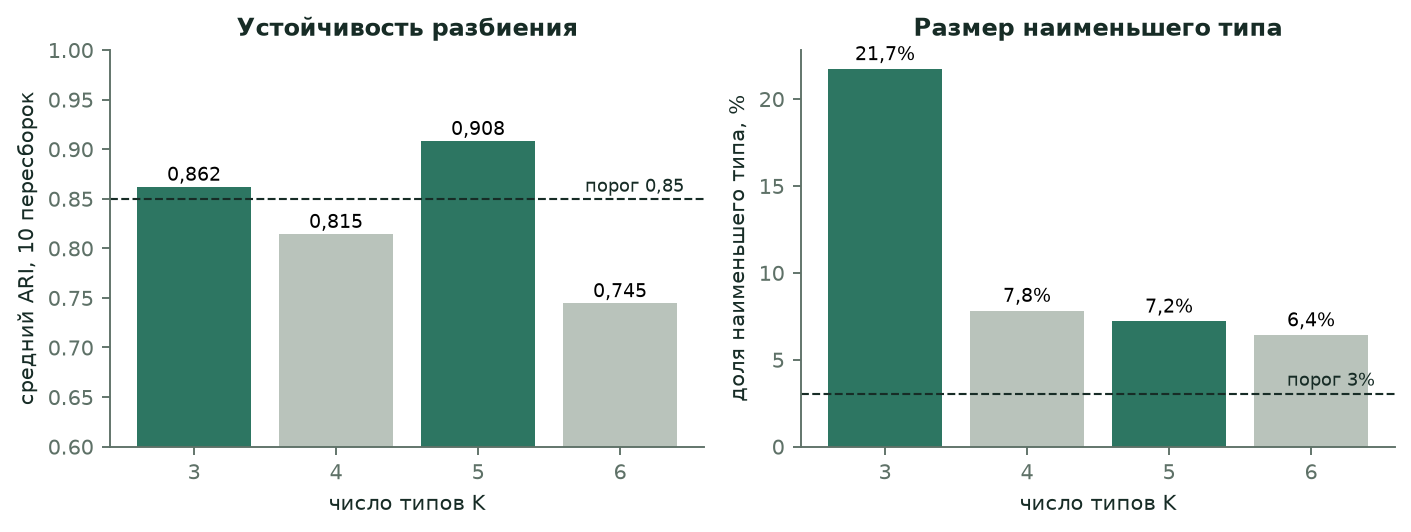
\includegraphics[width=0.94\linewidth]{figures/fig_k_selection.png}\caption*{Рис. 1. Выбор числа типов. Тёмно-зелёным отмечены допустимые K; пунктир
--- пороги протокола.}\end{figure}

\subsection{Параметры}\label{ux43fux430ux440ux430ux43cux435ux442ux440ux44b}

Параметры модели заданы в \texttt{configs/\allowbreak{}atlas.\allowbreak{}yaml}: число соседей \(k=15\) с минимумом три связи, один шаг сглаживания, штраф \(\tau = 0{,}5\) медианы, вес блока расходов 0,5, окно 12 месяцев, обрезка \(\pm 4\sigma\), seed 42. Влияние каждого параметра на результат оценено в разделе 9.3; результаты показывают, что отдельные параметры (вес блоков, сглаживание, длина окна, политика в отношении столиц) заметно меняют детальные границы типов.

\subsection{Границы применимости}\label{ux433ux440ux430ux43dux438ux446ux44b-ux43fux440ux438ux43cux435ux43dux438ux43cux43eux441ux442ux438}

Метод не предназначен для раннего обнаружения событий: сглаживание по сети и общие ретроспективные центры замедляют распознавание смены типа. Он не оценивает причины смен и не является прогнозной моделью (раздел 12).

\section{Индексы качества кластеризации (ICVI)}\label{ux438ux43dux434ux435ux43aux441ux44b-ux43aux430ux447ux435ux441ux442ux432ux430-ux43aux43bux430ux441ux442ux435ux440ux438ux437ux430ux446ux438ux438-icvi}

\subsection{Определения}\label{ux43eux43fux440ux435ux434ux435ux43bux435ux43dux438ux44f}

Использованы признаковые индексы (SW, CH, S\_Dbw) и графовые (AVI, AVU; Biswas, Biswas, 2017; MQ, ANUI и модулярность Q). AVI, AVU и MQ оценивают долю веса связей вершины (кластера), приходящуюся на свой или на чужой кластер; ANUI --- свёртка \(1/(\mathrm{AVU} + 1/\mathrm{AVI})\). Больше --- лучше для SW, CH, AVI, MQ, ANUI и Q; меньше --- лучше для S\_Dbw и AVU. Формулы приведены в приложении A.

\subsection{Реализация и проверка}\label{ux440ux435ux430ux43bux438ux437ux430ux446ux438ux44f-ux438-ux43fux440ux43eux432ux435ux440ux43aux430}

Все индексы реализованы заново и проверены автоматическими тестами: SW и CH --- против \texttt{scikit-\allowbreak{}learn}, модулярность --- против \texttt{igraph}, вершинные и попарные графовые индексы --- по допустимому диапазону и поведению на разбиениях с известной структурой. Графовые индексы вычисляются на симметричном графе без петель.

\subsection{Два определения графовых индексов}\label{ux434ux432ux430-ux43eux43fux440ux435ux434ux435ux43bux435ux43dux438ux44f-ux433ux440ux430ux444ux43eux432ux44bux445-ux438ux43dux434ux435ux43aux441ux43eux432}

В открытых реализациях (библиотека Pattern) AVI, AVU, ANUI и MQ определены \textbf{на уровне пар кластеров} (в таблицах --- индекс \texttt{\_\allowbreak{}ref}). При сбалансированных внедиагональных блоках AVU в такой форме определяется только числом кластеров, \(\mathrm{AVU}_{ref} = (K-1)/(2K-3)\), и не зависит от качества разбиения, а \(\mathrm{MQ}_{ref} = K \cdot \mathrm{AVI}_{ref}\) является перемасштабированием AVI. Рядом приведены \textbf{вершинные} определения (доля веса связей вершины, приходящаяся на свой кластер или на самый притягательный чужой, усреднённая по вершинам), у которых такого вырождения нет.

\Needspace*{11\baselineskip}\begingroup\footnotesize\setlength{\tabcolsep}{4pt}

{\def\LTcaptype{none} % do not increment counter
\begin{longtable}[]{@{}
  >{\raggedright\arraybackslash}p{(\linewidth - 10\tabcolsep) * \real{0.0450}}
  >{\raggedright\arraybackslash}p{(\linewidth - 10\tabcolsep) * \real{0.1802}}
  >{\raggedright\arraybackslash}p{(\linewidth - 10\tabcolsep) * \real{0.1261}}
  >{\raggedright\arraybackslash}p{(\linewidth - 10\tabcolsep) * \real{0.1351}}
  >{\raggedright\arraybackslash}p{(\linewidth - 10\tabcolsep) * \real{0.1712}}
  >{\raggedright\arraybackslash}p{(\linewidth - 10\tabcolsep) * \real{0.3423}}@{}}
\toprule\noalign{}
\begin{minipage}[b]{\linewidth}\raggedright
K
\end{minipage} & \begin{minipage}[b]{\linewidth}\raggedright
\(\mathrm{AVU}_{ref}\)
\end{minipage} & \begin{minipage}[b]{\linewidth}\raggedright
\((K-1)/(2K-3)\)
\end{minipage} & \begin{minipage}[b]{\linewidth}\raggedright
AVU (вершинный)
\end{minipage} & \begin{minipage}[b]{\linewidth}\raggedright
\(\mathrm{MQ}_{ref}\)
\end{minipage} & \begin{minipage}[b]{\linewidth}\raggedright
\(\mathrm{MQ}_{ref}/\mathrm{AVI}_{ref}\)
\end{minipage} \\
\midrule\noalign{}
\endhead
\bottomrule\noalign{}
\endlastfoot
3 & 0,667 & 0,667 & 0,076 & 2,777 & 3,00 \\
4 & 0,615 & 0,600 & 0,121 & 3,565 & 4,00 \\
5 & 0,580 & 0,571 & 0,118 & 4,416 & 5,00 \\
6 & 0,598 & 0,556 & 0,137 & 5,184 & 6,00 \\
\end{longtable}
}

\endgroup

На основной типологии эталонное значение AVU при каждом K лежит в пределах 0,05 от теоретического для сбалансированных блоков, тогда как вершинный AVU варьируется независимо от него. Поэтому в сравнении методов (раздел 7) приведены эталонные формулы для сопоставимости с принятой реализацией, а содержательные выводы опираются главным образом на признаковые индексы и вершинные варианты (приложение B).

\subsection{Значения для каждого K}\label{ux437ux43dux430ux447ux435ux43dux438ux44f-ux434ux43bux44f-ux43aux430ux436ux434ux43eux433ux43e-k}

\Needspace*{11\baselineskip}\begingroup\scriptsize\setlength{\tabcolsep}{4pt}

{\def\LTcaptype{none} % do not increment counter
\begin{longtable}[]{@{}
  >{\raggedright\arraybackslash}p{(\linewidth - 16\tabcolsep) * \real{0.0820}}
  >{\raggedright\arraybackslash}p{(\linewidth - 16\tabcolsep) * \real{0.1148}}
  >{\raggedright\arraybackslash}p{(\linewidth - 16\tabcolsep) * \real{0.1148}}
  >{\raggedright\arraybackslash}p{(\linewidth - 16\tabcolsep) * \real{0.1148}}
  >{\raggedright\arraybackslash}p{(\linewidth - 16\tabcolsep) * \real{0.1148}}
  >{\raggedright\arraybackslash}p{(\linewidth - 16\tabcolsep) * \real{0.1148}}
  >{\raggedright\arraybackslash}p{(\linewidth - 16\tabcolsep) * \real{0.1148}}
  >{\raggedright\arraybackslash}p{(\linewidth - 16\tabcolsep) * \real{0.1148}}
  >{\raggedright\arraybackslash}p{(\linewidth - 16\tabcolsep) * \real{0.1148}}@{}}
\toprule\noalign{}
\begin{minipage}[b]{\linewidth}\raggedright
K
\end{minipage} & \begin{minipage}[b]{\linewidth}\raggedright
SW
\end{minipage} & \begin{minipage}[b]{\linewidth}\raggedright
CH
\end{minipage} & \begin{minipage}[b]{\linewidth}\raggedright
S\_Dbw
\end{minipage} & \begin{minipage}[b]{\linewidth}\raggedright
AVI
\end{minipage} & \begin{minipage}[b]{\linewidth}\raggedright
AVU
\end{minipage} & \begin{minipage}[b]{\linewidth}\raggedright
ANUI
\end{minipage} & \begin{minipage}[b]{\linewidth}\raggedright
MQ
\end{minipage} & \begin{minipage}[b]{\linewidth}\raggedright
Q
\end{minipage} \\
\midrule\noalign{}
\endhead
\bottomrule\noalign{}
\endlastfoot
3 & 0,199 & 415,2 & 1,108 & 0,922 & 0,076 & 0,862 & 2,777 & 0,561 \\
4 & 0,134 & 339,6 & 0,772 & 0,874 & 0,121 & 0,790 & 3,565 & 0,594 \\
5 & 0,124 & 292,1 & 0,726 & 0,870 & 0,118 & 0,789 & 4,416 & 0,619 \\
6 & 0,098 & 256,8 & 0,698 & 0,852 & 0,137 & 0,763 & 5,184 & 0,655 \\
\end{longtable}
}

\endgroup

Сырые значения индексов нельзя сравнивать между разными \(K\): у случайного разбиения AVI убывает примерно как \(1/K\), а MQ растёт с \(K\).

\subsection{Значимость против нулевых моделей}\label{ux437ux43dux430ux447ux438ux43cux43eux441ux442ux44c-ux43fux440ux43eux442ux438ux432-ux43dux443ux43bux435ux432ux44bux445-ux43cux43eux434ux435ux43bux435ux439}

Для каждого индекса основной типологии (K = 5, окна декабрь 2023, июнь 2024, декабрь 2024) вычислено распределение по 200 нулевым разбиениям трёх видов: (а) \emph{перестановка меток} при сохранении размеров типов; (б) \emph{перестановка внутри регионов} при сохранении регионального состава типов --- проверяет, что структура не сводится к «просто регионам»; (в) \emph{перестройка рёбер} с сохранением степеней вершин и перестановкой весов (только графовые индексы). Знак z выбран так, что положительное значение означает «лучше нуля» (для S\_Dbw и AVU знак инвертирован); p --- односторонний эмпирический, его минимум \(1/(200+1)\).

\begingroup\small\setlength{\tabcolsep}{4pt}

{\def\LTcaptype{none} % do not increment counter
\begin{longtable}[]{@{}
  >{\raggedright\arraybackslash}p{(\linewidth - 6\tabcolsep) * \real{0.1839}}
  >{\raggedright\arraybackslash}p{(\linewidth - 6\tabcolsep) * \real{0.2874}}
  >{\raggedright\arraybackslash}p{(\linewidth - 6\tabcolsep) * \real{0.2529}}
  >{\raggedright\arraybackslash}p{(\linewidth - 6\tabcolsep) * \real{0.2759}}@{}}
\toprule\noalign{}
\begin{minipage}[b]{\linewidth}\raggedright
Индекс
\end{minipage} & \begin{minipage}[b]{\linewidth}\raggedright
Перестановка меток: z (p)
\end{minipage} & \begin{minipage}[b]{\linewidth}\raggedright
Внутри регионов: z (p)
\end{minipage} & \begin{minipage}[b]{\linewidth}\raggedright
Перестройка рёбер: z (p)
\end{minipage} \\
\midrule\noalign{}
\endhead
\bottomrule\noalign{}
\endlastfoot
SW & 27,1 (p ≤ 0,005) & 94,0 (p ≤ 0,005) & --- \\
CH & 946,4 (p ≤ 0,005) & 98,1 (p ≤ 0,005) & --- \\
S\_Dbw & 34,1 (p ≤ 0,005) & 42,6 (p ≤ 0,005) & --- \\
AVI (вершинный) & 133,5 (p ≤ 0,005) & 80,1 (p ≤ 0,005) & 118,1 (p ≤ 0,005) \\
AVU (вершинный) & 97,4 (p ≤ 0,005) & 68,2 (p ≤ 0,005) & 82,7 (p ≤ 0,005) \\
ANUI (вершинный) & 142,4 (p ≤ 0,005) & 93,1 (p ≤ 0,005) & 126,1 (p ≤ 0,005) \\
MQ (вершинный) & 110,1 (p ≤ 0,005) & 47,9 (p ≤ 0,005) & 112,1 (p ≤ 0,005) \\
Q & 98,6 (p ≤ 0,005) & 44,3 (p ≤ 0,005) & 100,7 (p ≤ 0,005) \\
AVI (эталон) & 110,1 (p ≤ 0,005) & 47,9 (p ≤ 0,005) & 112,1 (p ≤ 0,005) \\
AVU (эталон) & −17,2 (p = 1,000) & −26,0 (p = 1,000) & −37,4 (p = 1,000) \\
ANUI (эталон) & 77,9 (p ≤ 0,005) & 35,3 (p ≤ 0,005) & 79,5 (p ≤ 0,005) \\
MQ (эталон) & 110,1 (p ≤ 0,005) & 47,9 (p ≤ 0,005) & 112,1 (p ≤ 0,005) \\
\end{longtable}
}

\endgroup

В таблице приведены средние z по трём окнам и максимальное p. Для всех индексов, кроме эталонного AVU, наблюдаемое значение лучше любого из нулевых во всех окнах. Абсолютные z очень велики из-за малого разброса нулевых значений и не измеряют величину эффекта; важен знак и p. При перестановке внутри регионов z для большинства индексов меньше, чем при перестановке меток, но везде остаётся положительным: типы связаны не только с региональной принадлежностью. Эталонный AVU при всех трёх нулевых моделях оказывается \emph{хуже} нуля (z \textless{} 0): это подтверждает вырожденность определения на уровне пар кластеров (раздел 6.3). Результат для графовых индексов цикличен: граф использован при сглаживании, поэтому перестройка рёбер проверяет согласованность типов с конкретной структурой связей, но не даёт независимого подтверждения.

\subsection{Использование индексов}\label{ux438ux441ux43fux43eux43bux44cux437ux43eux432ux430ux43dux438ux435-ux438ux43dux434ux435ux43aux441ux43eux432}

Индексы применены для выбора числа типов (раздел 5.3), сравнения правил построения сети (раздел 4.3) и сравнения методов (раздел 7). Везде, где индекс вычисляется на сети, по которой построено разбиение или выполнено сглаживание, сравнение отчасти циклично: GS-TKM использует эту сеть при сглаживании, поэтому высокие значения графовых индексов у него ожидаемы. Графовые индексы коррелируют друг с другом и не складываются как независимые свидетельства. Значимость индексов проверена против нулевых моделей (раздел 6.5).

\section{Сравнение методов}\label{ux441ux440ux430ux432ux43dux435ux43dux438ux435-ux43cux435ux442ux43eux434ux43eux432}

\subsection{Участники}\label{ux443ux447ux430ux441ux442ux43dux438ux43aux438}

Сопоставлено 13 методов и вариантов на общих входах: стандартизованные признаки окна, общая сеть окна (раздел 4.1) и K = 5.

\begingroup\small\setlength{\tabcolsep}{4pt}

{\def\LTcaptype{none} % do not increment counter
\begin{longtable}[]{@{}
  >{\raggedright\arraybackslash}p{(\linewidth - 4\tabcolsep) * \real{0.3738}}
  >{\raggedright\arraybackslash}p{(\linewidth - 4\tabcolsep) * \real{0.2150}}
  >{\raggedright\arraybackslash}p{(\linewidth - 4\tabcolsep) * \real{0.4112}}@{}}
\toprule\noalign{}
\begin{minipage}[b]{\linewidth}\raggedright
Метод
\end{minipage} & \begin{minipage}[b]{\linewidth}\raggedright
Что использует
\end{minipage} & \begin{minipage}[b]{\linewidth}\raggedright
Описание
\end{minipage} \\
\midrule\noalign{}
\endhead
\bottomrule\noalign{}
\endlastfoot
k-means (срезы) & признаки & k-means в каждом окне отдельно, без сети и без временного регуляризатора \\
Ward (срезы) & признаки & агломеративная кластеризация по критерию Уорда \\
GMM diagonal (срезы) & признаки & смесь гауссиан с диагональной ковариацией \\
Spectral (срезы) & сеть & спектральная кластеризация по матрице смежности \\
Leiden (срезы) & сеть & оптимизация модулярности в каждом окне; разрешение подобрано под K на средней дате \\
Multilayer Leiden & сеть + время & модулярность на многослойной сети со связью между окнами \(\omega = 0{,}2\) \\
DMoN & признаки + сеть & графовая нейронная сеть, максимизирующая модулярность, 300 эпох \\
KEFRiN Euclidean, KEFRiN Cosine (авторы) & признаки + сеть & k-means, восстанавливающий признаки и строки матрицы связей (Shalileh, Mirkin, 2022); авторская реализация, бинарная смежность общей сети \\
CANUS (авторы) & признаки + сеть & градиентное обновление центров с фильтрацией вкладов по норме градиента; авторская реализация, 300 эпох \\
Общие центры, без сети & признаки & GS-TKM без сглаживания по сети (0 шагов) \\
GS-TKM без Витерби & признаки + сеть & GS-TKM с нулевым штрафом за смену типа \\
GS-TKM & признаки + сеть + время & основной метод (раздел 5) \\
\end{longtable}
}

\endgroup

Реализации KEFRiN и CANUS запускаются авторским кодом, закреплённым по коммиту и SHA-256; собственная реализация не подставляется. Для них повторная стандартизация KEFRiN отключена, чтобы сохранить веса блоков признаков.

\subsection{Протокол}\label{ux43fux440ux43eux442ux43eux43aux43eux43b}

Каждый метод оценивается на трёх датах (декабрь 2023, июнь 2024, декабрь 2024) при трёх значениях seed (42, 43, 44), то есть по девяти значениям каждого индекса; таблицы содержат средние. Статические методы работают на отдельных окнах, временные методы используют всю историю. Все индексы вычисляются в исходном стандартизованном пространстве признаков и на общей сети окна. Для каждого метода отдельно измерено согласие запусков: ARI между разбиениями последнего окна при разных seed. \textbf{Бюджеты настройки гиперпараметров не уравнены:} параметры сторонних методов фиксированы по рекомендациям авторов и не подбирались.

\subsection{Результаты}\label{ux440ux435ux437ux443ux43bux44cux442ux430ux442ux44b}

\begingroup\scriptsize\setlength{\tabcolsep}{4pt}

{\def\LTcaptype{none} % do not increment counter
\begin{longtable}[]{@{}
  >{\raggedright\arraybackslash}p{(\linewidth - 18\tabcolsep) * \real{0.2632}}
  >{\raggedright\arraybackslash}p{(\linewidth - 18\tabcolsep) * \real{0.0737}}
  >{\raggedright\arraybackslash}p{(\linewidth - 18\tabcolsep) * \real{0.0737}}
  >{\raggedright\arraybackslash}p{(\linewidth - 18\tabcolsep) * \real{0.0737}}
  >{\raggedright\arraybackslash}p{(\linewidth - 18\tabcolsep) * \real{0.0737}}
  >{\raggedright\arraybackslash}p{(\linewidth - 18\tabcolsep) * \real{0.0737}}
  >{\raggedright\arraybackslash}p{(\linewidth - 18\tabcolsep) * \real{0.0737}}
  >{\raggedright\arraybackslash}p{(\linewidth - 18\tabcolsep) * \real{0.0737}}
  >{\raggedright\arraybackslash}p{(\linewidth - 18\tabcolsep) * \real{0.0737}}
  >{\raggedright\arraybackslash}p{(\linewidth - 18\tabcolsep) * \real{0.1474}}@{}}
\toprule\noalign{}
\begin{minipage}[b]{\linewidth}\raggedright
Метод
\end{minipage} & \begin{minipage}[b]{\linewidth}\raggedright
SW
\end{minipage} & \begin{minipage}[b]{\linewidth}\raggedright
CH
\end{minipage} & \begin{minipage}[b]{\linewidth}\raggedright
S\_Dbw
\end{minipage} & \begin{minipage}[b]{\linewidth}\raggedright
AVI
\end{minipage} & \begin{minipage}[b]{\linewidth}\raggedright
AVU
\end{minipage} & \begin{minipage}[b]{\linewidth}\raggedright
ANUI
\end{minipage} & \begin{minipage}[b]{\linewidth}\raggedright
MQ
\end{minipage} & \begin{minipage}[b]{\linewidth}\raggedright
Q
\end{minipage} & \begin{minipage}[b]{\linewidth}\raggedright
ARI между seed
\end{minipage} \\
\midrule\noalign{}
\endhead
\bottomrule\noalign{}
\endlastfoot
Leiden (срезы) & 0,078 & 240,9 & 0,745 & 0,954 & 0,612 & 0,602 & 4,450 & 0,679 & 0,843 \\
Multilayer Leiden & 0,072 & 219,0 & 0,753 & 0,951 & 0,568 & 0,617 & 4,753 & 0,670 & 0,881 \\
Spectral (срезы) & 0,094 & 240,6 & 0,724 & 0,943 & 0,557 & 0,619 & 4,716 & 0,692 & 0,999 \\
DMoN & 0,057 & 234,5 & 0,716 & 0,909 & 0,681 & 0,562 & 4,546 & 0,689 & 0,725 \\
GS-TKM без Витерби & 0,119 & 286,0 & 0,727 & 0,891 & 0,595 & 0,582 & 4,453 & 0,640 & 0,995 \\
\textbf{GS-TKM} & 0,120 & 287,1 & 0,727 & 0,890 & 0,605 & 0,579 & 4,452 & 0,641 & 0,993 \\
KEFRiN Cosine (авторы) & 0,115 & 284,9 & 0,691 & 0,840 & 0,615 & 0,554 & 4,200 & 0,611 & 0,717 \\
KEFRiN Euclidean (авторы) & 0,135 & 318,7 & 0,717 & 0,792 & 0,564 & 0,547 & 3,959 & 0,587 & 0,832 \\
CANUS (авторы) & 0,105 & 271,1 & 0,710 & 0,732 & 0,606 & 0,507 & 3,660 & 0,534 & 0,582 \\
Общие центры, без сети & 0,142 & 322,3 & 0,716 & 0,723 & 0,564 & 0,514 & 3,615 & 0,529 & 0,988 \\
k-means (срезы) & 0,141 & 323,9 & 0,719 & 0,719 & 0,556 & 0,514 & 3,597 & 0,529 & 0,959 \\
Ward (срезы) & 0,120 & 254,2 & 0,787 & 0,642 & 0,521 & 0,482 & 3,209 & 0,431 & 1,000 \\
GMM diagonal (срезы) & 0,113 & 285,0 & 0,775 & 0,594 & 0,605 & 0,437 & 2,968 & 0,429 & 0,796 \\
\end{longtable}
}

\endgroup

Индексы AVI, AVU, ANUI, MQ в таблице --- эталонные формулы (уровень пар кластеров); вершинные определения и Q приведены в приложении B. SW и CH --- больше лучше, S\_Dbw и AVU --- меньше лучше.

\begin{figure}[H]\centering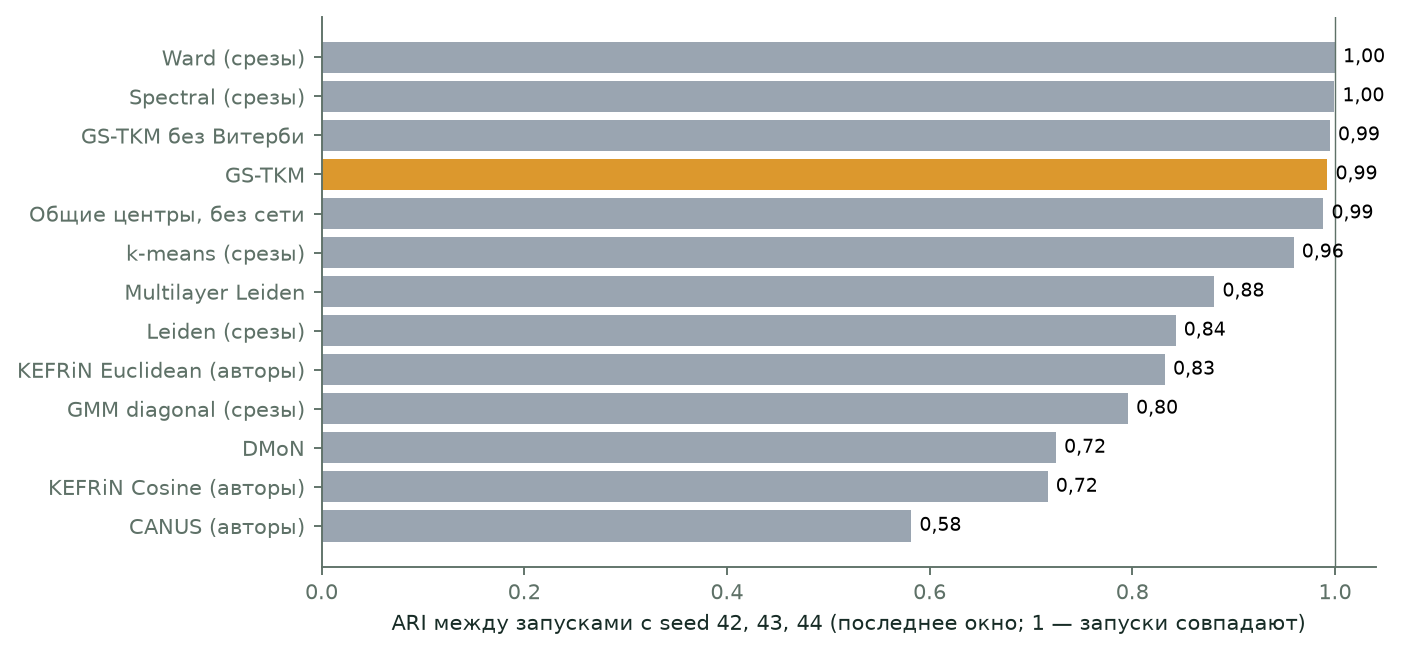
\includegraphics[width=0.94\linewidth]{figures/fig_seed_agreement.png}\caption*{Рис. 2. Согласие между запусками с seed 42, 43, 44 (ARI, последнее
окно). Выделен GS-TKM.}\end{figure}

\subsection{Интерпретация}\label{ux438ux43dux442ux435ux440ux43fux440ux435ux442ux430ux446ux438ux44f}

GS-TKM не занимает первых мест по индексам: лучший по эталонному AVI --- «Leiden (срезы)» (0,954), лучший по SW --- «Общие центры, без сети» (0,142); у GS-TKM AVI = 0,890 и SW = 0,120. По сравнению с k-means на срезах сглаживание повышает AVI с 0,719 до 0,890 и снижает SW с 0,141 до 0,120: признаковая компактность отдаётся за согласованность с сетью. Методы, оптимизирующие модулярность (Leiden, спектральный, многослойный Leiden), выигрывают по графовым индексам, но по SW и CH уступают методам на признаках. Согласие запусков с разными seed у GS-TKM высокое (0,993) и сопоставимо с Ward (1,000), спектральным методом (0,999) и k-means (0,959), но выше, чем у KEFRiN Euclidean (0,832), KEFRiN Cosine (0,717), DMoN (0,725) и CANUS (0,582). Метки GS-TKM согласованы между окнами по построению (общие центры), чего нет у методов, запускаемых на срезах. Штраф за смену типа почти не меняет оценки по отдельным окнам (AVI 0,890 и 0,891 без него): он влияет на траектории между окнами, а индексы вычисляются внутри окна.

\subsection{Ограничения сравнения}\label{ux43eux433ux440ux430ux43dux438ux447ux435ux43dux438ux44f-ux441ux440ux430ux432ux43dux435ux43dux438ux44f}

\begin{itemize}
\tightlist
\item
  Бюджеты настройки не равны, параметры сторонних методов не подбирались под данные; результаты для KEFRiN, CANUS и DMoN не следует считать их предельным качеством.
\item
  Графовые индексы вычисляются на сети, которую использует GS-TKM; методы, не использующие сеть, оцениваются на ней заведомо менее выгодно.
\item
  Для каждого метода по три даты и три seed; интервалы на места методов не строились.
\item
  Метки статических методов в соседних окнах не согласованы между собой, поэтому динамические свойства (число смен типа) для них не сравниваются.
\end{itemize}

\subsection{Синтетические данные с известной истиной}\label{ux441ux438ux43dux442ux435ux442ux438ux447ux435ux441ux43aux438ux435-ux434ux430ux43dux43dux44bux435-ux441-ux438ux437ux432ux435ux441ux442ux43dux43eux439-ux438ux441ux442ux438ux43dux43eux439}

Внутренние индексы и устойчивость к подвыборкам не отвечают на главный вопрос динамической типологии: отличает ли метод настоящую смену типа от шума. Для этого использован генератор динамических сетей с известной истиной: \(N = 600\) узлов, \(K = 5\) сообществ, \(T = 12\) окон, 7 признаков; признак \(y_{it} = \mu_{k(i,t)} + u_i + \varepsilon_{it}\) (центр сообщества, устойчивый эффект узла и шум), в окне 6 доля 15\% узлов меняет сообщество, плюс фоновая смена 1\% в окно. Сеть --- стохастическая блочная модель по текущему составу с персистентностью рёбер 0,7 либо граф ближайших соседей. Шесть режимов проверяют допущения метода:

\begin{itemize}
\tightlist
\item
  \textbf{fe} --- устойчивые эффекты узлов (\(\sigma_u = 0{,}66\)) и слабый шум (\(\sigma_\varepsilon = 0{,}28\));
\item
  \textbf{no\_fe} --- эффектов узлов нет;
\item
  \textbf{highnoise} --- шум втрое выше;
\item
  \textbf{drift} --- центры сообществ дрейфуют во времени;
\item
  \textbf{knn\_graph} --- сеть строится как kNN по тем же шумным признакам, то есть так же, как в реальной обработке;
\item
  \textbf{comp\_graph} --- сеть строится по другому, независимому шумному сигналу о тех же сообществах (сеть «знает» то, чего нет в признаках).
\end{itemize}

Метрики: NMI к истине (среднее по окнам); доля настоящих мигрантов, распознанных в месяц смены и через два месяца; доля ложных смен (узел-окно, где метод сменил метку, а истина не менялась). Хорош метод с высокой распознаваемостью при низкой доле ложных смен; одну стабильность метод может «купить», запретив смены. Значения --- среднее по 5 реализациям генератора.

\begingroup\footnotesize\setlength{\tabcolsep}{4pt}

{\def\LTcaptype{none} % do not increment counter
\begin{longtable}[]{@{}
  >{\raggedright\arraybackslash}p{(\linewidth - 10\tabcolsep) * \real{0.1111}}
  >{\raggedright\arraybackslash}p{(\linewidth - 10\tabcolsep) * \real{0.2778}}
  >{\raggedright\arraybackslash}p{(\linewidth - 10\tabcolsep) * \real{0.0648}}
  >{\raggedright\arraybackslash}p{(\linewidth - 10\tabcolsep) * \real{0.2222}}
  >{\raggedright\arraybackslash}p{(\linewidth - 10\tabcolsep) * \real{0.2130}}
  >{\raggedright\arraybackslash}p{(\linewidth - 10\tabcolsep) * \real{0.1111}}@{}}
\toprule\noalign{}
\begin{minipage}[b]{\linewidth}\raggedright
Режим
\end{minipage} & \begin{minipage}[b]{\linewidth}\raggedright
Метод
\end{minipage} & \begin{minipage}[b]{\linewidth}\raggedright
NMI
\end{minipage} & \begin{minipage}[b]{\linewidth}\raggedright
Мигранты (в месяц смены)
\end{minipage} & \begin{minipage}[b]{\linewidth}\raggedright
Мигранты (через 2 мес.)
\end{minipage} & \begin{minipage}[b]{\linewidth}\raggedright
Ложные смены
\end{minipage} \\
\midrule\noalign{}
\endhead
\bottomrule\noalign{}
\endlastfoot
fe & \textbf{GS-TKM} & 0,885 & 0,26 & 0,80 & 0,026 \\
& GS-TKM без штрафа & 0,863 & 0,28 & 0,78 & 0,049 \\
& GS-TKM без сглаживания по сети & 0,646 & 0,83 & 0,82 & 0,011 \\
& k-means по окнам & 0,601 & 0,82 & 0,80 & 0,150 \\
& Leiden по сети & 0,902 & 0,08 & 0,82 & 0,019 \\
no\_fe & \textbf{GS-TKM} & 0,916 & 0,29 & 0,85 & 0,021 \\
& GS-TKM без штрафа & 0,911 & 0,29 & 0,84 & 0,026 \\
& GS-TKM без сглаживания по сети & 0,997 & 1,00 & 0,98 & 0,001 \\
& k-means по окнам & 0,989 & 1,00 & 0,97 & 0,007 \\
& Leiden по сети & 0,902 & 0,08 & 0,82 & 0,019 \\
highnoise & \textbf{GS-TKM} & 0,848 & 0,28 & 0,76 & 0,043 \\
& GS-TKM без штрафа & 0,783 & 0,30 & 0,71 & 0,112 \\
& GS-TKM без сглаживания по сети & 0,484 & 0,68 & 0,76 & 0,104 \\
& k-means по окнам & 0,317 & 0,58 & 0,60 & 0,473 \\
& Leiden по сети & 0,902 & 0,08 & 0,82 & 0,019 \\
drift & \textbf{GS-TKM} & 0,618 & 0,24 & 0,50 & 0,352 \\
& GS-TKM без штрафа & 0,587 & 0,30 & 0,47 & 0,454 \\
& GS-TKM без сглаживания по сети & 0,571 & 0,64 & 0,65 & 0,186 \\
& k-means по окнам & 0,827 & 0,97 & 0,96 & 0,104 \\
& Leiden по сети & 0,901 & 0,10 & 0,83 & 0,019 \\
knn\_graph & \textbf{GS-TKM} & 0,630 & 0,82 & 0,81 & 0,042 \\
& GS-TKM без штрафа & 0,587 & 0,79 & 0,80 & 0,154 \\
& GS-TKM без сглаживания по сети & 0,646 & 0,83 & 0,82 & 0,011 \\
& k-means по окнам & 0,601 & 0,82 & 0,80 & 0,150 \\
& Leiden по сети & 0,573 & 0,75 & 0,79 & 0,118 \\
comp\_graph & \textbf{GS-TKM} & 0,875 & 0,94 & 0,92 & 0,084 \\
& GS-TKM без штрафа & 0,853 & 0,93 & 0,91 & 0,104 \\
& GS-TKM без сглаживания по сети & 0,646 & 0,83 & 0,82 & 0,011 \\
& k-means по окнам & 0,601 & 0,82 & 0,80 & 0,150 \\
& Leiden по сети & 0,891 & 0,93 & 0,94 & 0,071 \\
\end{longtable}
}

\endgroup

Выводы:

\begin{enumerate}
\def\labelenumi{\arabic{enumi}.}
\tightlist
\item
  \textbf{Сеть помогает там, где она несёт дополнительную информацию.} В режиме comp\_graph NMI GS-TKM равен 0,875 против 0,646 без графового сглаживания. В режиме knn\_graph, где сеть построена из тех же признаков (как в реальной обработке), выигрыша нет: 0,630 против 0,646. Поэтому польза графового сглаживания на реальных данных не гарантируется; её нельзя выводить из роста графовых индексов (раздел 13).
\item
  \textbf{Штраф за смену снижает ложные смены без потери распознавания.} В режиме knn\_graph доля ложных смен падает с 0,154 (без штрафа) до 0,042 при близкой распознаваемости мигрантов.
\item
  \textbf{Распознавание запаздывает.} В режиме fe GS-TKM распознаёт 0,26 мигрантов в месяц смены и 0,80 через два месяца: сглаживание и штраф замедляют реакцию (раздел 5.5).
\item
  \textbf{Дрейф центров --- слабое место.} В режиме drift NMI GS-TKM равен 0,618, а k-means по окнам с венгерским сопоставлением даёт 0,827: общие центры предполагают неподвижные центры типов. Это согласуется с наблюдаемым на реальных данных общим сдвигом потребления (раздел 9.4).
\item
  \textbf{Без эффектов узлов графовое сглаживание вредит.} В режиме no\_fe NMI GS-TKM --- 0,916 против 0,997 без сглаживания.
\end{enumerate}

Синтетическая проверка не доказывает качества на реальных данных: она показывает, в каких условиях допущения метода выполняются, и в каких режимах он проигрывает более простым вариантам.

\section{Типология и её интерпретация}\label{ux442ux438ux43fux43eux43bux43eux433ux438ux44f-ux438-ux435ux451-ux438ux43dux442ux435ux440ux43fux440ux435ux442ux430ux446ux438ux44f}

\subsection{Пять типов}\label{ux43fux44fux442ux44c-ux442ux438ux43fux43eux432}

Основная типология содержит 5 типов для 1~776 территорий. Названия присвоены по правилам из \texttt{semantic\_\allowbreak{}names} (порядок проверки: уровень расходов, затем ресурсная и промышленная доли занятости, затем доля государственного сектора) по профилям декабря 2024 года и сохраняются на всей траектории; они описывают центр типа, а не каждую территорию.

\Needspace*{13\baselineskip}\begingroup\scriptsize\setlength{\tabcolsep}{4pt}

{\def\LTcaptype{none} % do not increment counter
\begin{longtable}[]{@{}
  >{\raggedright\arraybackslash}p{(\linewidth - 18\tabcolsep) * \real{0.0435}}
  >{\raggedright\arraybackslash}p{(\linewidth - 18\tabcolsep) * \real{0.3652}}
  >{\raggedright\arraybackslash}p{(\linewidth - 18\tabcolsep) * \real{0.0435}}
  >{\raggedright\arraybackslash}p{(\linewidth - 18\tabcolsep) * \real{0.1130}}
  >{\raggedright\arraybackslash}p{(\linewidth - 18\tabcolsep) * \real{0.1217}}
  >{\raggedright\arraybackslash}p{(\linewidth - 18\tabcolsep) * \real{0.0609}}
  >{\raggedright\arraybackslash}p{(\linewidth - 18\tabcolsep) * \real{0.0696}}
  >{\raggedright\arraybackslash}p{(\linewidth - 18\tabcolsep) * \real{0.0609}}
  >{\raggedright\arraybackslash}p{(\linewidth - 18\tabcolsep) * \real{0.0609}}
  >{\raggedright\arraybackslash}p{(\linewidth - 18\tabcolsep) * \real{0.0609}}@{}}
\toprule\noalign{}
\begin{minipage}[b]{\linewidth}\raggedright
Тип
\end{minipage} & \begin{minipage}[b]{\linewidth}\raggedright
Название
\end{minipage} & \begin{minipage}[b]{\linewidth}\raggedright
МО
\end{minipage} & \begin{minipage}[b]{\linewidth}\raggedright
Расходы, руб.
\end{minipage} & \begin{minipage}[b]{\linewidth}\raggedright
Зарплата, руб.
\end{minipage} & \begin{minipage}[b]{\linewidth}\raggedright
Еда
\end{minipage} & \begin{minipage}[b]{\linewidth}\raggedright
Общеп.
\end{minipage} & \begin{minipage}[b]{\linewidth}\raggedright
Марк.
\end{minipage} & \begin{minipage}[b]{\linewidth}\raggedright
Пром.
\end{minipage} & \begin{minipage}[b]{\linewidth}\raggedright
Гос.
\end{minipage} \\
\midrule\noalign{}
\endhead
\bottomrule\noalign{}
\endlastfoot
1 & Низкие расходы, продовольственный профиль & 564 & 22~094 & 40~952 & 48,0\% & 1,3\% & 18,6\% & 0,0\% & 57,4\% \\
2 & Смешанная занятость и средние расходы & 461 & 26~636 & 50~458 & 44,8\% & 2,5\% & 17,1\% & 8,0\% & 45,6\% \\
3 & Промышленность и сервисное потребление & 339 & 35~670 & 63~930 & 38,2\% & 5,2\% & 14,6\% & 18,9\% & 35,8\% \\
4 & Государственный сектор и умеренные расходы & 284 & 23~928 & 46~376 & 45,4\% & 2,2\% & 14,6\% & 0,0\% & 60,8\% \\
5 & Высокий уровень расходов и зарплат & 128 & 39~634 & 103~083 & 42,8\% & 3,6\% & 10,6\% & 0,7\% & 40,4\% \\
\end{longtable}
}

\endgroup

Расходы --- рубли на жителя в месяц (медиана по типу, среднее за последнее окно), зарплата --- рубли в месяц (по данным Росстата за 2023 год), столбцы «Еда», «Общеп.», «Марк.» --- доли еды, общепита и маркетплейсов в расходах, столбцы «Пром.» и «Гос.» --- нижние границы раскрытых долей занятости в промышленности и в государственном секторе (неопубликованные ячейки заменены нулём, поэтому нуль означает «не раскрыто», а не «отсутствует»). Доля добывающих отраслей в медианах всех типов равна нулю и в таблицу не включена.

Содержательно типы читаются так.

\begin{itemize}
\tightlist
\item
  \textbf{Низкие расходы, продовольственный профиль} (\(n=564\)): самые низкие расходы на жителя, наибольшая доля продовольствия и самые низкие зарплаты.
\item
  \textbf{Смешанная занятость и средние расходы} (\(n=461\)): средний уровень расходов, раскрытая доля промышленности около 8\%.
\item
  \textbf{Промышленность и сервисное потребление} (\(n=339\)): повышенные расходы, наибольшая доля общепита и наибольшая раскрытая промышленная занятость.
\item
  \textbf{Государственный сектор и умеренные расходы} (\(n=284\)): расходы выше нижнего типа, наибольшая раскрытая доля государственного сектора.
\item
  \textbf{Высокий уровень расходов и зарплат} (\(n=128\)): наибольшие расходы и зарплаты.
\end{itemize}

Показатели занятости неполны: нижние границы раскрытых долей не позволяют надёжно различать отрасли там, где значения скрыты, поэтому названия «Промышленность\ldots» и «Государственный сектор\ldots» следует понимать как «среди раскрытых данных».

\begin{figure}[H]\centering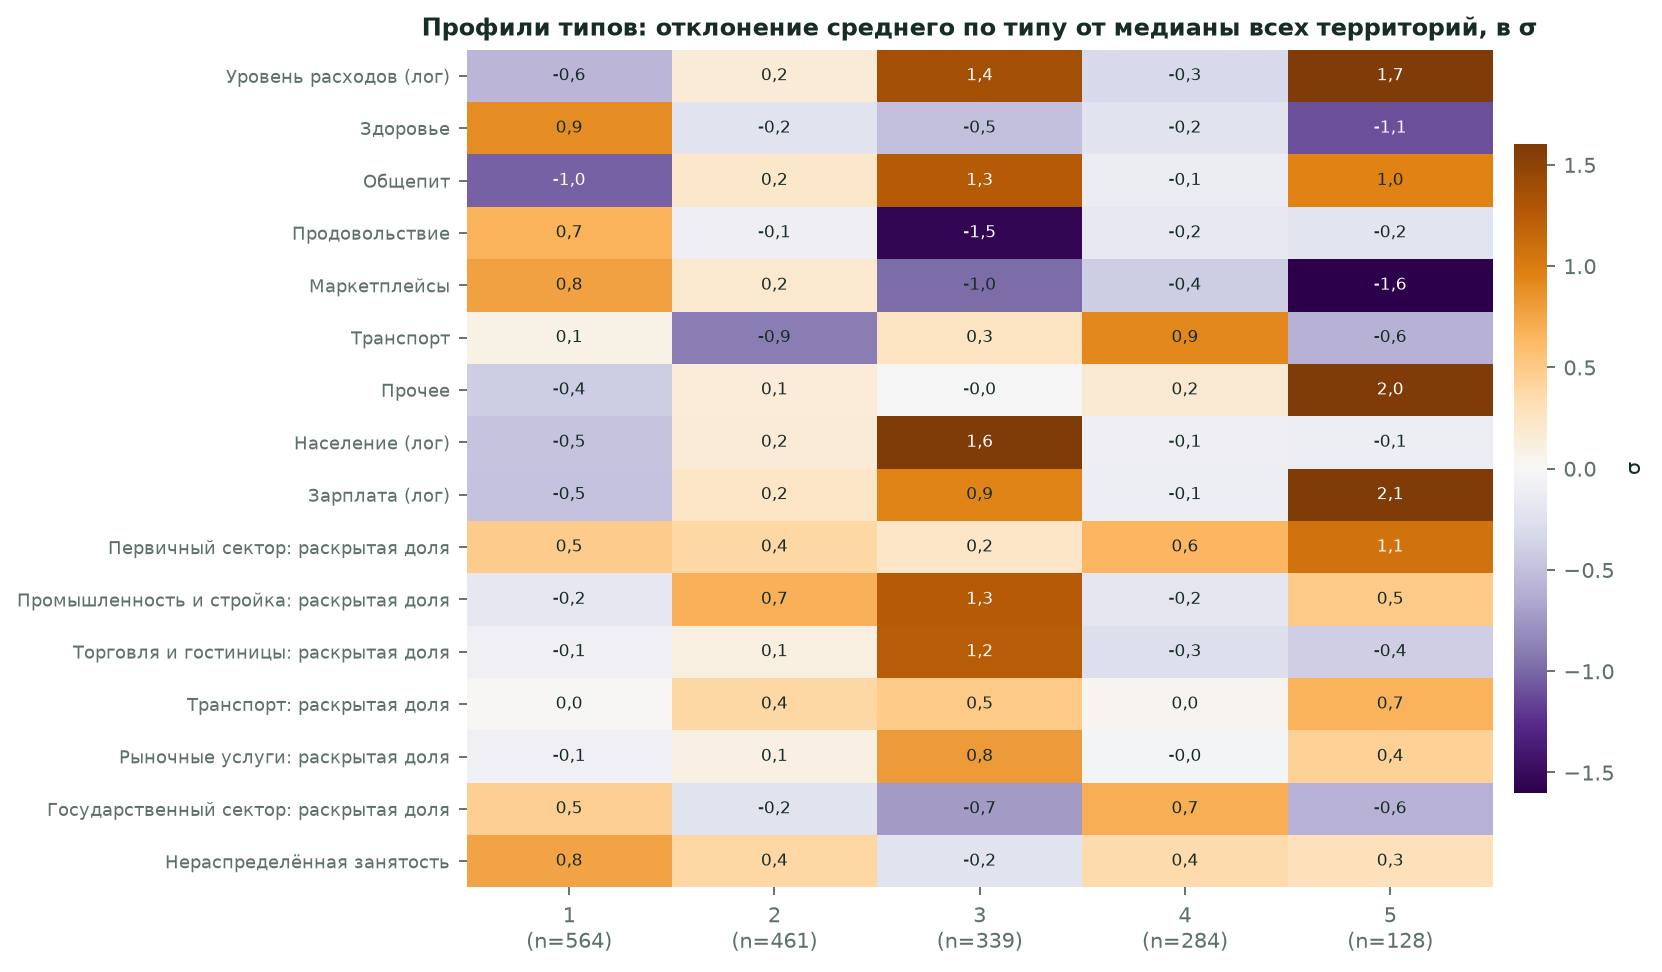
\includegraphics[width=0.94\linewidth]{figures/fig_profiles.png}\caption*{Рис. 3. Отклонение средних значений признаков типа от медианы всех
территорий (в единицах σ), декабрь 2024.}\end{figure}

\subsection{Карта}\label{ux43aux430ux440ux442ux430}

\begin{figure}[H]\centering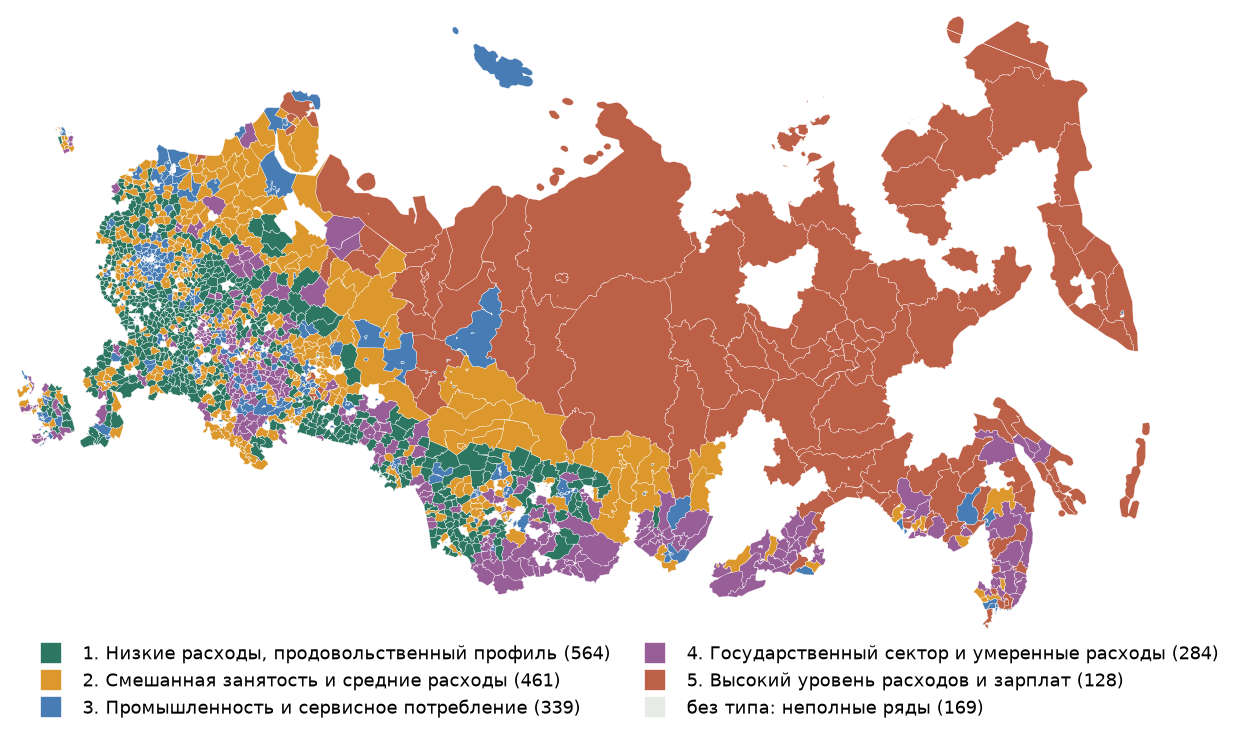
\includegraphics[width=0.94\linewidth]{figures/fig_map.png}\caption*{Рис. 4. Типы территорий в декабре 2024 (цвета соответствуют рис. 3).
Территории с неполной историей показаны светлым цветом.}\end{figure}

\subsection{Три разбиения разной детальности}\label{ux442ux440ux438-ux440ux430ux437ux431ux438ux435ux43dux438ux44f-ux440ux430ux437ux43dux43eux439-ux434ux435ux442ux430ux43bux44cux43dux43eux441ux442ux438}

K = 3, 4, 5 рассчитаны независимо. Согласие разбиений K = 3 и K = 4 с основным (ARI) и размер наименьшего типа приведены в таблице; разбиения не образуют иерархию: тип K = 4 может делиться между несколькими типами K = 5.

\Needspace*{9\baselineskip}\begingroup\small\setlength{\tabcolsep}{4pt}

{\def\LTcaptype{none} % do not increment counter
\begin{longtable}[]{@{}
  >{\raggedright\arraybackslash}p{(\linewidth - 4\tabcolsep) * \real{0.1064}}
  >{\raggedright\arraybackslash}p{(\linewidth - 4\tabcolsep) * \real{0.6596}}
  >{\raggedright\arraybackslash}p{(\linewidth - 4\tabcolsep) * \real{0.2340}}@{}}
\toprule\noalign{}
\begin{minipage}[b]{\linewidth}\raggedright
K
\end{minipage} & \begin{minipage}[b]{\linewidth}\raggedright
Наименьший тип в последнем окне
\end{minipage} & \begin{minipage}[b]{\linewidth}\raggedright
ARI с K = 5
\end{minipage} \\
\midrule\noalign{}
\endhead
\bottomrule\noalign{}
\endlastfoot
3 & 21,7\% & 0,388 \\
4 & 7,8\% & 0,677 \\
5 & 7,2\% & 1,000 \\
\end{longtable}
}

\endgroup

\subsection{Две линзы}\label{ux434ux432ux435-ux43bux438ux43dux437ux44b-1}

Помимо общей линзы построена линза потребления (только блок расходов; раздел 3.5). Согласие меток двух линз --- ARI 0,614. Линза потребления нужна для внешней проверки (раздел 11): показатели контекста (зарплата, население) проверяются только на ней, так как в общей линзе они входят в признаки.

\section{Устойчивость и неопределённость}\label{ux443ux441ux442ux43eux439ux447ux438ux432ux43eux441ux442ux44c-ux438-ux43dux435ux43eux43fux440ux435ux434ux435ux43bux451ux43dux43dux43eux441ux442ux44c}

\subsection{Устойчивость отдельных типов}\label{ux443ux441ux442ux43eux439ux447ux438ux432ux43eux441ux442ux44c-ux43eux442ux434ux435ux43bux44cux43dux44bux445-ux442ux438ux43fux43eux432}

Разбиение пересобрано 50 раз на случайных подвыборках из 80\% территорий (без возвращения; на каждой пересборке заново обучаются преобразования, сеть и центры); метки пересобранных моделей сопоставлены с основными по венгерскому алгоритму. Для каждого типа вычислен коэффициент Жаккара между исходным множеством и ближайшим пересобранным (критерий Хеннига: значение ниже 0,6 говорит о нестабильном типе, выше 0,75 --- о стабильном, выше 0,85 --- о высокой устойчивости).

\Needspace*{13\baselineskip}\begingroup\footnotesize\setlength{\tabcolsep}{4pt}

{\def\LTcaptype{none} % do not increment counter
\begin{longtable}[]{@{}
  >{\raggedright\arraybackslash}p{(\linewidth - 10\tabcolsep) * \real{0.0500}}
  >{\raggedright\arraybackslash}p{(\linewidth - 10\tabcolsep) * \real{0.4200}}
  >{\raggedright\arraybackslash}p{(\linewidth - 10\tabcolsep) * \real{0.0500}}
  >{\raggedright\arraybackslash}p{(\linewidth - 10\tabcolsep) * \real{0.1600}}
  >{\raggedright\arraybackslash}p{(\linewidth - 10\tabcolsep) * \real{0.1900}}
  >{\raggedright\arraybackslash}p{(\linewidth - 10\tabcolsep) * \real{0.1300}}@{}}
\toprule\noalign{}
\begin{minipage}[b]{\linewidth}\raggedright
Тип
\end{minipage} & \begin{minipage}[b]{\linewidth}\raggedright
Название
\end{minipage} & \begin{minipage}[b]{\linewidth}\raggedright
МО
\end{minipage} & \begin{minipage}[b]{\linewidth}\raggedright
Жаккар (среднее)
\end{minipage} & \begin{minipage}[b]{\linewidth}\raggedright
Диапазон пересборок
\end{minipage} & \begin{minipage}[b]{\linewidth}\raggedright
ARI (среднее)
\end{minipage} \\
\midrule\noalign{}
\endhead
\bottomrule\noalign{}
\endlastfoot
1 & Низкие расходы, продовольственный профиль & 564 & 0,943 & {[}0,90; 0,97{]} & 0,893 \\
2 & Смешанная занятость и средние расходы & 461 & 0,899 & {[}0,83; 0,94{]} & 0,893 \\
3 & Промышленность и сервисное потребление & 339 & 0,920 & {[}0,88; 0,95{]} & 0,893 \\
4 & Государственный сектор и умеренные расходы & 284 & 0,881 & {[}0,76; 0,93{]} & 0,893 \\
5 & Высокий уровень расходов и зарплат & 128 & 0,901 & {[}0,81; 0,96{]} & 0,893 \\
\end{longtable}
}

\endgroup

Минимальное среднее значение Жаккара --- 0,881 (тип «Государственный сектор и умеренные расходы»); все типы превышают порог 0,85.

\subsection{Устойчивость разбиения в целом}\label{ux443ux441ux442ux43eux439ux447ux438ux432ux43eux441ux442ux44c-ux440ux430ux437ux431ux438ux435ux43dux438ux44f-ux432-ux446ux435ux43bux43eux43c}

Средний ARI между пересобранными и основным разбиениями равен 0,893 (95-процентный интервал по пересборкам --- от 0,831 до 0,926). Для K = 3 и K = 4 значения составляют 0,862 и 0,841. Дополнительно приведено обычное сопоставление «основное разбиение против 10 пересборок» (таблица в разделе 5.3), по которому выбиралось K.

\begin{figure}[H]\centering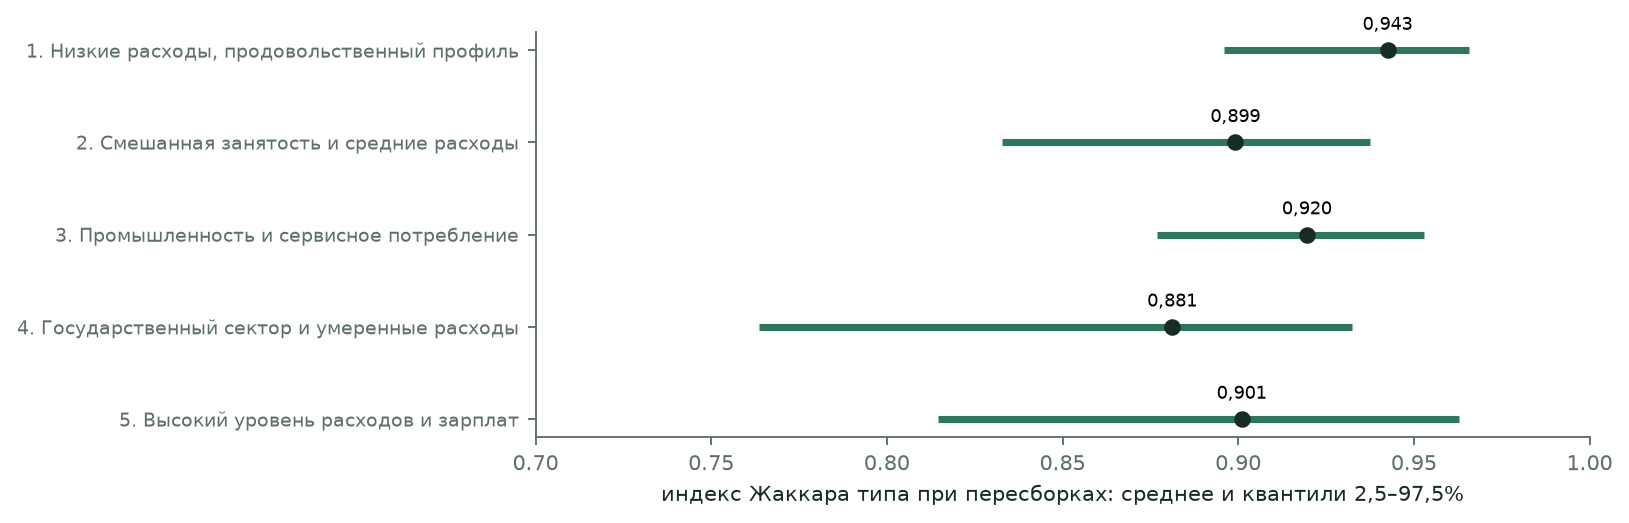
\includegraphics[width=0.94\linewidth]{figures/fig_bootstrap.png}\caption*{Рис. 5. Устойчивость типов при пересборке на 80\% территорий: среднее
значение Жаккара и диапазон по 50 пересборкам.}\end{figure}

\subsection{Чувствительность к параметрам}\label{ux447ux443ux432ux441ux442ux432ux438ux442ux435ux43bux44cux43dux43eux441ux442ux44c-ux43a-ux43fux430ux440ux430ux43cux435ux442ux440ux430ux43c}

Каждый параметр меняется по отдельности, остальные фиксированы. В таблице: ARI между результирующей и основной последней меткой и доля территорий, сменивших тип за 2024 год («изменившиеся»).

\begingroup\small\setlength{\tabcolsep}{4pt}

{\def\LTcaptype{none} % do not increment counter
\begin{longtable}[]{@{}
  >{\raggedright\arraybackslash}p{(\linewidth - 6\tabcolsep) * \real{0.3663}}
  >{\raggedright\arraybackslash}p{(\linewidth - 6\tabcolsep) * \real{0.2772}}
  >{\raggedright\arraybackslash}p{(\linewidth - 6\tabcolsep) * \real{0.2475}}
  >{\raggedright\arraybackslash}p{(\linewidth - 6\tabcolsep) * \real{0.1089}}@{}}
\toprule\noalign{}
\begin{minipage}[b]{\linewidth}\raggedright
Параметр
\end{minipage} & \begin{minipage}[b]{\linewidth}\raggedright
Значение
\end{minipage} & \begin{minipage}[b]{\linewidth}\raggedright
ARI с основной типологией
\end{minipage} & \begin{minipage}[b]{\linewidth}\raggedright
Сменили тип
\end{minipage} \\
\midrule\noalign{}
\endhead
\bottomrule\noalign{}
\endlastfoot
Вес блока расходов & 0,25 & 0,641 & 15,5\% \\
Вес блока расходов & 0,5 & 1,000 & 16,9\% \\
Вес блока расходов & 0,75 & 0,721 & 21,1\% \\
Число соседей & 8 & 0,929 & 17,3\% \\
Число соседей & 15 & 1,000 & 16,9\% \\
Число соседей & 30 & 0,925 & 18,3\% \\
Шаги сглаживания & 0 & 0,575 & 6,0\% \\
Шаги сглаживания & 1 & 1,000 & 16,9\% \\
Шаги сглаживания & 2 & 0,911 & 18,6\% \\
Штраф (доли медианы) & 0 & 0,855 & 26,2\% \\
Штраф (доли медианы) & 0,5 & 1,000 & 16,9\% \\
Штраф (доли медианы) & 1,0 & 0,939 & 12,4\% \\
Seed k-means & 1 & 0,999 & 17,0\% \\
Seed k-means & 2 & 0,983 & 16,7\% \\
Seed k-means & 3 & 0,999 & 17,1\% \\
Seed k-means & 4 & 0,968 & 17,3\% \\
Seed k-means & 5 & 0,982 & 16,8\% \\
Координата неопубликованной занятости & исключена & 0,923 & 17,5\% \\
Столицы & внутригородские МО раздельно & 0,513 & 14,3\% \\
Столицы & столицы исключены & 0,946 & 17,5\% \\
Длина окна, мес. & 3 & 0,648 & 42,1\% \\
Вычет медианы по территориям & только уровень расходов & 0,917 & 16,5\% \\
Вычет медианы по территориям & все координаты расходов & 0,792 & 7,8\% \\
\end{longtable}
}

\endgroup

\begin{figure}[H]\centering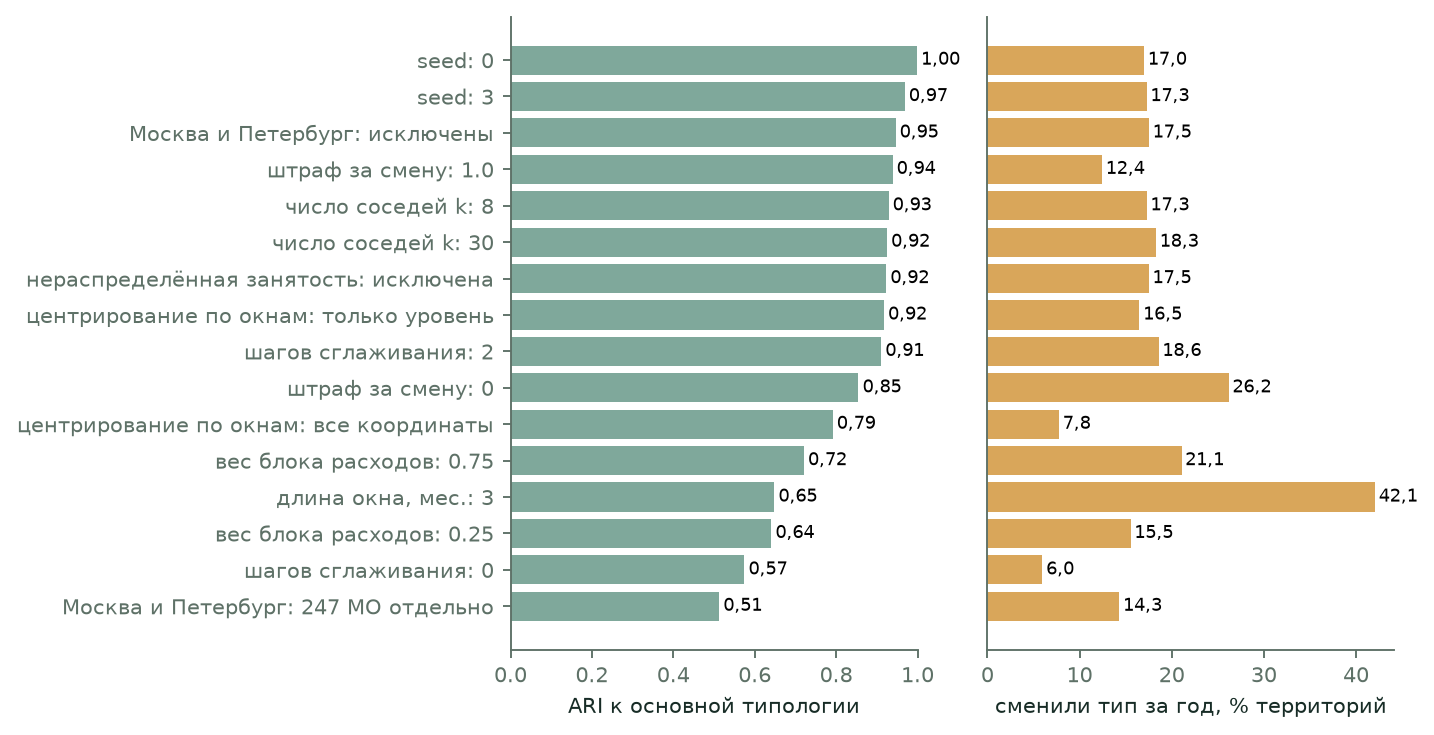
\includegraphics[width=0.94\linewidth]{figures/fig_sensitivity.png}\caption*{Рис. 6. ARI с основной типологией при изменении параметров.}\end{figure}

Выводы по таблице:

\begin{enumerate}
\def\labelenumi{\arabic{enumi}.}
\tightlist
\item
  \textbf{Вес блоков} (0,25 и 0,75) меняет детальные границы (ARI 0,641 и 0,721); результат нельзя считать независимым от выбора 50/50. Равный вес выбран как нейтральное значение, а не подбирался под критерий.
\item
  \textbf{Сглаживание.} Без сглаживания (0 шагов) ARI составляет 0,575; это самый сильный эффект среди параметров метода. Сеть заметно меняет границы типов.
\item
  \textbf{Штраф.} Без штрафа за смену типа доля изменивших тип растёт с 16,9\% до 26,2\%, при двойном штрафе падает до 12,4\%; штраф регулирует баланс между гибкостью и стабильностью траектории.
\item
  \textbf{Число соседей, seed и исключение координаты неопубликованной занятости} (ARI не ниже 0,92) слабо влияют на метки.
\item
  \textbf{Политика в отношении столиц.} Если оставить 247 внутригородских МО без объединения, ARI на оставшихся территориях падает до 0,51: внутригородские единицы заметно искажают общие центры. Простое исключение столиц даёт ARI 0,95.
\item
  \textbf{Длина окна.} Квартальные окна (3 месяца) дают ARI 0,65 и долю изменивших тип 42,1\%: короткое окно захватывает сезонность и шум.
\end{enumerate}

\subsection{Общий сдвиг потребления}\label{ux43eux431ux449ux438ux439-ux441ux434ux432ux438ux433-ux43fux43eux442ux440ux435ux431ux43bux435ux43dux438ux44f}

Часть смен типа обусловлена общей для всех территорий динамикой номинальных расходов и доли маркетплейсов. Если из каждого окна вычесть медиану признаков расходов (по территориям), то доля изменивших тип снижается с 16,9\% до 7,8\% (ARI с основной типологией --- 0,79); если вычесть медиану только из логарифма уровня, доля равна 16,5\% (ARI 0,92).

\begin{figure}[H]\centering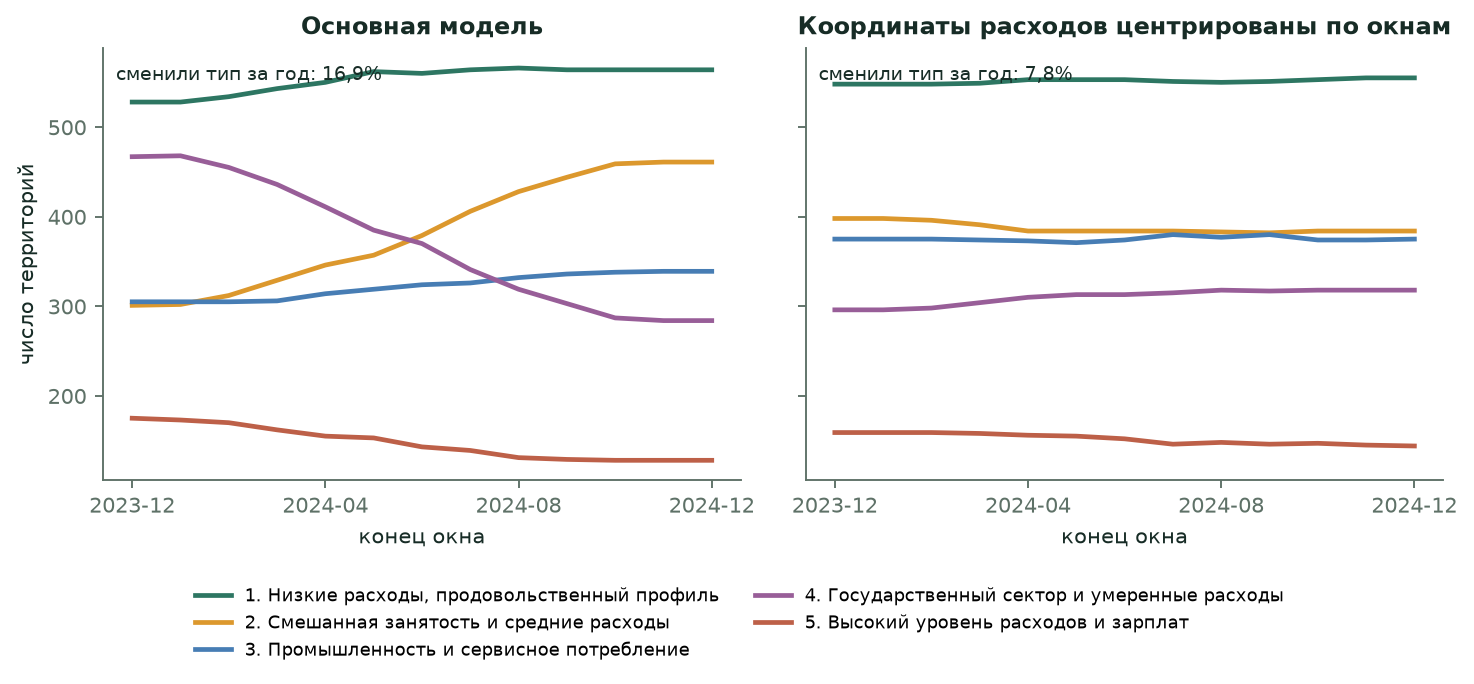
\includegraphics[width=0.94\linewidth]{figures/fig_drift.png}\caption*{Рис. 7. Доля изменивших тип за 2024 год до и после центрирования окон.}\end{figure}

Поэтому тип «изменился» нельзя без оговорки читать как «территория изменилась относительно прочих»: заметная часть смен отражает, что вся страна смещается относительно центров, обученных на всех окнах.

\subsection{Неопределённость отнесения каждой территории}\label{ux43dux435ux43eux43fux440ux435ux434ux435ux43bux451ux43dux43dux43eux441ux442ux44c-ux43eux442ux43dux435ux441ux435ux43dux438ux44f-ux43aux430ux436ux434ux43eux439-ux442ux435ux440ux440ux438ux442ux43eux440ux438ux438}

Для каждой территории и окна хранятся две величины. \textbf{Согласие при пересборке} --- доля пересборок, в которых территория получила тот же тип (в декабре 2024: медиана 1,00, у 87,3\% территорий не ниже 0,9, у 2,3\% ниже 0,5). Это характеристика процедуры, а не вероятность истинного типа. \textbf{Знаковый запас} --- разность между расстоянием до ближайшего чужого центра и расстоянием до назначенного; отрицательное значение (у 5,7\% территорий в последнем окне) допустимо, поскольку траектория выбирается с учётом штрафа, а не по ближайшему центру.

\section{Динамика типов}\label{ux434ux438ux43dux430ux43cux438ux43aux430-ux442ux438ux43fux43eux432}

\subsection{Переходы}\label{ux43fux435ux440ux435ux445ux43eux434ux44b}

За 2024 год (12 переходов между окнами 13 срезов) зафиксировано 317 смен типа у 303 территорий (17,1\% от 1~776; часть территорий меняет тип более одного раза). Матрица переходов:

\Needspace*{13\baselineskip}\begingroup\footnotesize\setlength{\tabcolsep}{4pt}

{\def\LTcaptype{none} % do not increment counter
\begin{longtable}[]{@{}
  >{\raggedright\arraybackslash}p{(\linewidth - 12\tabcolsep) * \real{0.5789}}
  >{\raggedright\arraybackslash}p{(\linewidth - 12\tabcolsep) * \real{0.0658}}
  >{\raggedright\arraybackslash}p{(\linewidth - 12\tabcolsep) * \real{0.0658}}
  >{\raggedright\arraybackslash}p{(\linewidth - 12\tabcolsep) * \real{0.0658}}
  >{\raggedright\arraybackslash}p{(\linewidth - 12\tabcolsep) * \real{0.0658}}
  >{\raggedright\arraybackslash}p{(\linewidth - 12\tabcolsep) * \real{0.0658}}
  >{\raggedright\arraybackslash}p{(\linewidth - 12\tabcolsep) * \real{0.0921}}@{}}
\toprule\noalign{}
\begin{minipage}[b]{\linewidth}\raggedright
Из ~в
\end{minipage} & \begin{minipage}[b]{\linewidth}\raggedright
1
\end{minipage} & \begin{minipage}[b]{\linewidth}\raggedright
2
\end{minipage} & \begin{minipage}[b]{\linewidth}\raggedright
3
\end{minipage} & \begin{minipage}[b]{\linewidth}\raggedright
4
\end{minipage} & \begin{minipage}[b]{\linewidth}\raggedright
5
\end{minipage} & \begin{minipage}[b]{\linewidth}\raggedright
Всего
\end{minipage} \\
\midrule\noalign{}
\endhead
\bottomrule\noalign{}
\endlastfoot
1 (Низкие расходы, продовольственный профиль) & --- & 42 & 0 & 2 & 0 & 44 \\
2 (Смешанная занятость и средние расходы) & 3 & --- & 10 & 0 & 2 & 15 \\
3 (Промышленность и сервисное потребление) & 0 & 8 & --- & 1 & 1 & 10 \\
4 (Государственный сектор и умеренные расходы) & 77 & 97 & 14 & --- & 5 & 193 \\
5 (Высокий уровень расходов и зарплат) & 0 & 28 & 20 & 7 & --- & 55 \\
\end{longtable}
}

\endgroup

Строки --- исходный тип, столбцы --- новый (нумерация с единицы). Крупнейшие потоки: из типа 4 в тип 2 (97 смен), из типа 4 в тип 1 (77) и из типа 1 в тип 2 (42); вместе они составляют 68\% всех смен. Эти направления нужно читать с учётом общего сдвига потребления (раздел 9.4): движение территорий между соседними типами не обязательно означает изменение их положения относительно прочих территорий. Из типа 4 уходит 61\% всех смен; при пересборке на подвыборках наименьшее среднее значение Жаккара (0,881) имеет тип 4.

\subsection{Устойчивость новой метки}\label{ux443ux441ux442ux43eux439ux447ux438ux432ux43eux441ux442ux44c-ux43dux43eux432ux43eux439-ux43cux435ux442ux43aux438}

Смена считается \emph{устойчивой в описательном смысле}, если новая метка сохраняется как минимум на трёх конечных точках, нижняя граница совместного согласия четырёх меток (по неравенству объединения) не ниже 0,75 и знаковый запас неотрицателен. Из 317 смен критерию удовлетворяют 12:

\begingroup\footnotesize\setlength{\tabcolsep}{4pt}

{\def\LTcaptype{none} % do not increment counter
\begin{longtable}[]{@{}
  >{\raggedright\arraybackslash}p{(\linewidth - 14\tabcolsep) * \real{0.3364}}
  >{\raggedright\arraybackslash}p{(\linewidth - 14\tabcolsep) * \real{0.2091}}
  >{\raggedright\arraybackslash}p{(\linewidth - 14\tabcolsep) * \real{0.0818}}
  >{\raggedright\arraybackslash}p{(\linewidth - 14\tabcolsep) * \real{0.0455}}
  >{\raggedright\arraybackslash}p{(\linewidth - 14\tabcolsep) * \real{0.0455}}
  >{\raggedright\arraybackslash}p{(\linewidth - 14\tabcolsep) * \real{0.0909}}
  >{\raggedright\arraybackslash}p{(\linewidth - 14\tabcolsep) * \real{0.0636}}
  >{\raggedright\arraybackslash}p{(\linewidth - 14\tabcolsep) * \real{0.1273}}@{}}
\toprule\noalign{}
\begin{minipage}[b]{\linewidth}\raggedright
Территория
\end{minipage} & \begin{minipage}[b]{\linewidth}\raggedright
Регион
\end{minipage} & \begin{minipage}[b]{\linewidth}\raggedright
Месяц
\end{minipage} & \begin{minipage}[b]{\linewidth}\raggedright
Из
\end{minipage} & \begin{minipage}[b]{\linewidth}\raggedright
В
\end{minipage} & \begin{minipage}[b]{\linewidth}\raggedright
Согласие
\end{minipage} & \begin{minipage}[b]{\linewidth}\raggedright
Запас
\end{minipage} & \begin{minipage}[b]{\linewidth}\raggedright
Нижняя граница
\end{minipage} \\
\midrule\noalign{}
\endhead
\bottomrule\noalign{}
\endlastfoot
муниципальный округ Частинский & Пермский край & 2024-10 & 4 & 1 & 0,98 & 0,07 & 0,95 \\
городской округ Артинский & Свердловская область & 2024-10 & 4 & 1 & 0,93 & 0,34 & 0,91 \\
Руднянский муниципальный район & Смоленская область & 2024-03 & 4 & 1 & 0,98 & 0,24 & 0,90 \\
муниципальный округ Вилегодский & Архангельская область & 2024-06 & 4 & 2 & 0,90 & 0,05 & 0,90 \\
городской округ Карпинск & Свердловская область & 2024-03 & 5 & 2 & 1,00 & 0,19 & 0,85 \\
Колпашевский муниципальный район & Томская область & 2024-05 & 4 & 2 & 0,95 & 0,07 & 0,85 \\
Большеулуйский муниципальный район & Красноярский край & 2024-08 & 1 & 2 & 0,82 & 0,04 & 0,83 \\
Слободо-Туринский муниципальный район & Свердловская область & 2024-06 & 4 & 2 & 0,87 & 0,03 & 0,82 \\
Татарский муниципальный район & Новосибирская область & 2024-02 & 4 & 2 & 0,93 & 0,05 & 0,80 \\
Мотыгинский муниципальный район & Красноярский край & 2024-07 & 5 & 2 & 0,97 & 0,14 & 0,78 \\
городской округ Мамоновский & Калининградская область & 2024-08 & 4 & 2 & 0,82 & 0,05 & 0,77 \\
муниципальный округ Верхнекамский & Кировская область & 2024-02 & 4 & 1 & 0,98 & 0,13 & 0,76 \\
\end{longtable}
}

\endgroup

Эти 12 смен --- список для дополнительного изучения; причинность они не устанавливают. Последние два окна цензурированы (у них нет подтверждающих точек), поэтому смены в конце года попадают в список реже.

\subsection{Что динамика показывает и чего не показывает}\label{ux447ux442ux43e-ux434ux438ux43dux430ux43cux438ux43aux430-ux43fux43eux43aux430ux437ux44bux432ux430ux435ux442-ux438-ux447ux435ux433ux43e-ux43dux435-ux43fux43eux43aux430ux437ux44bux432ux430ux435ux442}

Динамика отражает смещение признаков относительно общих центров, а не причину. Метод не отделяет структурную смену от сезонности и общего дрейфа и не оценивает момент смены точнее, чем на масштаб месяцев (годовое скользящее окно смазывает момент). Пространственную диффузию (распространение смен по дорогам и соседям) в настоящей версии не проверяли.

\section{Внешняя проверка}\label{ux432ux43dux435ux448ux43dux44fux44f-ux43fux440ux43eux432ux435ux440ux43aux430}

\subsection{Протокол}\label{ux43fux440ux43eux442ux43eux43aux43eux43b-1}

Для каждой линзы проверяется, добавляет ли тип объясняющую силу сверх региональных фиксированных эффектов: разность скорректированного \(R^2\) линейной модели «внешний показатель по региону и типу» и «по региону». Интервалы строятся бутстрепом по регионам (200 повторов), значимость оценивается перестановками типов внутри регионов (499 перестановок) с поправкой Бенджамини--Хохберга по всем показателям. Затем показатели дополнительно контролируются логарифмами населения и зарплаты (чтобы тип не просто пересказывал размер территории).

Внешние показатели не входят в построение проверяемой линзы: для обеих линз проверяются показатели Росстата и доступность рынков, не входящие ни в один из блоков признаков; зарплата и население входят в контекстный блок, поэтому для них проверяется только линза потребления.

\subsection{Результаты}\label{ux440ux435ux437ux443ux43bux44cux442ux430ux442ux44b-1}

\begingroup\footnotesize\setlength{\tabcolsep}{4pt}

{\def\LTcaptype{none} % do not increment counter
\begin{longtable}[]{@{}
  >{\raggedright\arraybackslash}p{(\linewidth - 10\tabcolsep) * \real{0.0667}}
  >{\raggedright\arraybackslash}p{(\linewidth - 10\tabcolsep) * \real{0.2370}}
  >{\raggedright\arraybackslash}p{(\linewidth - 10\tabcolsep) * \real{0.0444}}
  >{\raggedright\arraybackslash}p{(\linewidth - 10\tabcolsep) * \real{0.2741}}
  >{\raggedright\arraybackslash}p{(\linewidth - 10\tabcolsep) * \real{0.0519}}
  >{\raggedright\arraybackslash}p{(\linewidth - 10\tabcolsep) * \real{0.3259}}@{}}
\toprule\noalign{}
\begin{minipage}[b]{\linewidth}\raggedright
Линза
\end{minipage} & \begin{minipage}[b]{\linewidth}\raggedright
Показатель
\end{minipage} & \begin{minipage}[b]{\linewidth}\raggedright
МО
\end{minipage} & \begin{minipage}[b]{\linewidth}\raggedright
\(\Delta\bar R^2\) {[}интервал по регионам{]}
\end{minipage} & \begin{minipage}[b]{\linewidth}\raggedright
q (BH)
\end{minipage} & \begin{minipage}[b]{\linewidth}\raggedright
После контроля населения и зарплаты {[}интервал{]}
\end{minipage} \\
\midrule\noalign{}
\endhead
\bottomrule\noalign{}
\endlastfoot
Общая & Доступность рынков (лог) & 1764 & 0,0116 {[}0,0067; 0,0217{]} & 0,002 & 0,0024 {[}0,0009; 0,0054{]} \\
Общая & Оборот торговли / житель, 2024 & 1514 & 0,1988 {[}0,1530; 0,2703{]} & 0,002 & 0,0071 {[}0,0027; 0,0182{]} \\
Общая & Оборот общепита / житель, 2024 & 1102 & 0,1233 {[}0,0802; 0,1782{]} & 0,002 & 0,0032 {[}−0,0007; 0,0198{]} \\
Общая & Ввод жилья / житель, 2024 & 1463 & 0,1230 {[}0,0880; 0,1713{]} & 0,002 & 0,0395 {[}0,0178; 0,0715{]} \\
Общая & Инвестиции / житель, 2023 & 1631 & 0,1027 {[}0,0710; 0,1511{]} & 0,002 & 0,0015 {[}−0,0005; 0,0080{]} \\
Общая & Гостиничные места / житель, 2024 & 965 & 0,0001 {[}−0,0023; 0,0115{]} & 0,368 & 0,0039 {[}−0,0026; 0,0263{]} \\
Потреб. & Доступность рынков (лог) & 1764 & 0,0095 {[}0,0054; 0,0158{]} & 0,002 & 0,0014 {[}0,0005; 0,0035{]} \\
Потреб. & Оборот торговли / житель, 2024 & 1514 & 0,1577 {[}0,1179; 0,2188{]} & 0,002 & 0,0027 {[}0,0001; 0,0170{]} \\
Потреб. & Оборот общепита / житель, 2024 & 1102 & 0,1019 {[}0,0654; 0,1512{]} & 0,002 & 0,0056 {[}0,0006; 0,0235{]} \\
Потреб. & Ввод жилья / житель, 2024 & 1463 & 0,1083 {[}0,0768; 0,1455{]} & 0,002 & 0,0300 {[}0,0156; 0,0557{]} \\
Потреб. & Инвестиции / житель, 2023 & 1631 & 0,0782 {[}0,0518; 0,1255{]} & 0,002 & −0,0005 {[}−0,0009; 0,0048{]} \\
Потреб. & Гостиничные места / житель, 2024 & 965 & −0,0015 {[}−0,0033; 0,0081{]} & 0,678 & 0,0079 {[}−0,0007; 0,0358{]} \\
Потреб. & Зарплата (лог), 2023 & 1776 & 0,0871 {[}0,0602; 0,1304{]} & 0,002 & --- \\
Потреб. & Население (лог), 2023 & 1744 & 0,3498 {[}0,2817; 0,4248{]} & 0,002 & --- \\
\end{longtable}
}

\endgroup

Добавочная объясняющая сила \(\Delta\bar R^2\) имеет региональный интервал целиком выше нуля для 5 из 6 показателей общей линзы. После контроля населения и зарплаты она резко падает: доступность рынков (лог) --- 0,0024; оборот торговли / житель --- 0,0071; оборот общепита / житель --- 0,0032; ввод жилья / житель --- 0,0395; инвестиции / житель --- 0,0015; гостиничные места / житель --- 0,0039. Значительная часть связи типа с внешними показателями объясняется размером и уровнем оплаты труда территории; остаточное добавление мало, но у 3 показателей его интервал не содержит нуль.

Показатель «гостиничные места на жителя» не проходит проверку: интервал включает ноль. Он оставлен в таблице как отрицательный результат.

\subsection{Ограничения}\label{ux43eux433ux440ux430ux43dux438ux447ux435ux43dux438ux44f}

Показатели Росстата с неполным покрытием (торговля --- 85\% территорий) относятся к крупным и средним организациям, поэтому для малых территорий они смещены. Региональные фиксированные эффекты поглощают значительную часть пространственной зависимости, но не всю; p-значения перестановок описательные.

\section{Проверка переноса и неполные истории}\label{ux43fux440ux43eux432ux435ux440ux43aux430-ux43fux435ux440ux435ux43dux43eux441ux430-ux438-ux43dux435ux43fux43eux43bux43dux44bux435-ux438ux441ux442ux43eux440ux438ux438}

\subsection{Практическая проверка: прогноз роста}\label{ux43fux440ux430ux43aux442ux438ux447ux435ux441ux43aux430ux44f-ux43fux440ux43eux432ux435ux440ux43aux430-ux43fux440ux43eux433ux43dux43eux437-ux440ux43eux441ux442ux430}

Проверено, помогает ли тип предсказывать рост логарифма расходов на жителя в 2024 году по признакам 2023 года. Сопоставлены модели «регион», «регион + признаки», «регион + признаки + тип» (гребневая регрессия, \(\alpha=10\)) и нелинейная модель (градиентный бустинг на гистограммах) при двух схемах кросс-валидации: случайные МО и регионы целиком. Все преобразования, сеть и типы строятся внутри фолда.

\begingroup\small\setlength{\tabcolsep}{4pt}

{\def\LTcaptype{none} % do not increment counter
\begin{longtable}[]{@{}
  >{\raggedright\arraybackslash}p{(\linewidth - 6\tabcolsep) * \real{0.2113}}
  >{\raggedright\arraybackslash}p{(\linewidth - 6\tabcolsep) * \real{0.4507}}
  >{\raggedright\arraybackslash}p{(\linewidth - 6\tabcolsep) * \real{0.2254}}
  >{\raggedright\arraybackslash}p{(\linewidth - 6\tabcolsep) * \real{0.1127}}@{}}
\toprule\noalign{}
\begin{minipage}[b]{\linewidth}\raggedright
Схема
\end{minipage} & \begin{minipage}[b]{\linewidth}\raggedright
Модель
\end{minipage} & \begin{minipage}[b]{\linewidth}\raggedright
MAE, лог. пункты
\end{minipage} & \begin{minipage}[b]{\linewidth}\raggedright
\(R^2\)
\end{minipage} \\
\midrule\noalign{}
\endhead
\bottomrule\noalign{}
\endlastfoot
МО случайно & Регион & 0,0245 & 0,171 \\
МО случайно & Регион + признаки & 0,0218 & 0,313 \\
МО случайно & Регион + признаки + тип & 0,0217 & 0,322 \\
МО случайно & Нелинейный контроль по признакам & 0,0220 & 0,293 \\
Регионы целиком & Регион & 0,0273 & −0,010 \\
Регионы целиком & Регион + признаки & 0,0240 & 0,163 \\
Регионы целиком & Регион + признаки + тип & 0,0239 & 0,170 \\
Регионы целиком & Нелинейный контроль по признакам & 0,0242 & 0,159 \\
\end{longtable}
}

\endgroup

Тип не даёт устойчивого выигрыша: прирост MAE от добавления типа --- для схемы «регионы целиком» 0,0001 лог. пункта (интервал {[}−0,0001; 0,0004{]}); интервал включает ноль. Тип полезен как описание и средство поиска аналогов, но не как прогнозный признак.

\subsection{Присвоение типа территориям с неполной историей}\label{ux43fux440ux438ux441ux432ux43eux435ux43dux438ux435-ux442ux438ux43fux430-ux442ux435ux440ux440ux438ux442ux43eux440ux438ux44fux43c-ux441-ux43dux435ux43fux43eux43bux43dux43eux439-ux438ux441ux442ux43eux440ux438ux435ux439}

Для 169 территорий с неполным периодом наблюдений полная модель не применяется. Индуктивное расширение использует одношаговое сглаживание по сети от полных территорий и присваивает тип ближайшего центра, если полное календарное окно 2024 года наблюдается и знаковый запас не ниже 0,15. Из них 20 получили предварительный тип.

Калибровка: для 200 полных территорий, исключённых из обучения модели, история обрезана до \(m\) месяцев, тип присвоен тем же способом и сопоставлен с полной моделью; территории разбиты на фолды по регионам (\texttt{GroupKFold}, 5 фолдов).

\Needspace*{11\baselineskip}\begingroup\footnotesize\setlength{\tabcolsep}{4pt}

{\def\LTcaptype{none} % do not increment counter
\begin{longtable}[]{@{}
  >{\raggedright\arraybackslash}p{(\linewidth - 12\tabcolsep) * \real{0.1442}}
  >{\raggedright\arraybackslash}p{(\linewidth - 12\tabcolsep) * \real{0.0481}}
  >{\raggedright\arraybackslash}p{(\linewidth - 12\tabcolsep) * \real{0.0962}}
  >{\raggedright\arraybackslash}p{(\linewidth - 12\tabcolsep) * \real{0.1346}}
  >{\raggedright\arraybackslash}p{(\linewidth - 12\tabcolsep) * \real{0.1058}}
  >{\raggedright\arraybackslash}p{(\linewidth - 12\tabcolsep) * \real{0.2500}}
  >{\raggedright\arraybackslash}p{(\linewidth - 12\tabcolsep) * \real{0.2212}}@{}}
\toprule\noalign{}
\begin{minipage}[b]{\linewidth}\raggedright
Месяцев истории
\end{minipage} & \begin{minipage}[b]{\linewidth}\raggedright
МО
\end{minipage} & \begin{minipage}[b]{\linewidth}\raggedright
Покрытие
\end{minipage} & \begin{minipage}[b]{\linewidth}\raggedright
Согласие (все)
\end{minipage} & \begin{minipage}[b]{\linewidth}\raggedright
Присвоено
\end{minipage} & \begin{minipage}[b]{\linewidth}\raggedright
Согласие среди присвоенных
\end{minipage} & \begin{minipage}[b]{\linewidth}\raggedright
Нижняя граница Вильсона
\end{minipage} \\
\midrule\noalign{}
\endhead
\bottomrule\noalign{}
\endlastfoot
6 & 200 & 77,5\% & 80,5\% & 155 & 87,1\% & 80,9\% \\
9 & 200 & 77,5\% & 81,5\% & 155 & 91,0\% & 85,4\% \\
12 & 200 & 77,0\% & 85,0\% & 154 & 92,2\% & 86,9\% \\
18 & 200 & 77,0\% & 85,0\% & 154 & 92,2\% & 86,9\% \\
\end{longtable}
}

\endgroup

Согласие со «своей» полной моделью при 12 месяцах среди присвоенных равно 92,2\% (нижняя граница Вильсона 86,9\%). Это согласие с ретроспективной моделью, а не вероятность истинного типа. Разбиение \texttt{GroupKFold} зависит от версии scikit-learn: при версии 1.9.1 согласие составляет 90,4\% вместо 92,2\%.

\section{Вклад сети}\label{ux432ux43aux43bux430ux434-ux441ux435ux442ux438}

Вклад сети оценивается тремя способами: сравнением «общие центры без сети» с GS-TKM (одинаковые центры и штраф, но без сглаживания), чувствительностью к числу шагов сглаживания (раздел 9.3) и сравнением правил построения сети (раздел 4.3).

\Needspace*{9\baselineskip}\begingroup\footnotesize\setlength{\tabcolsep}{4pt}

{\def\LTcaptype{none} % do not increment counter
\begin{longtable}[]{@{}
  >{\raggedright\arraybackslash}p{(\linewidth - 14\tabcolsep) * \real{0.2821}}
  >{\raggedright\arraybackslash}p{(\linewidth - 14\tabcolsep) * \real{0.0897}}
  >{\raggedright\arraybackslash}p{(\linewidth - 14\tabcolsep) * \real{0.0897}}
  >{\raggedright\arraybackslash}p{(\linewidth - 14\tabcolsep) * \real{0.0897}}
  >{\raggedright\arraybackslash}p{(\linewidth - 14\tabcolsep) * \real{0.0897}}
  >{\raggedright\arraybackslash}p{(\linewidth - 14\tabcolsep) * \real{0.0897}}
  >{\raggedright\arraybackslash}p{(\linewidth - 14\tabcolsep) * \real{0.0897}}
  >{\raggedright\arraybackslash}p{(\linewidth - 14\tabcolsep) * \real{0.1795}}@{}}
\toprule\noalign{}
\begin{minipage}[b]{\linewidth}\raggedright
Вариант
\end{minipage} & \begin{minipage}[b]{\linewidth}\raggedright
SW
\end{minipage} & \begin{minipage}[b]{\linewidth}\raggedright
CH
\end{minipage} & \begin{minipage}[b]{\linewidth}\raggedright
S\_Dbw
\end{minipage} & \begin{minipage}[b]{\linewidth}\raggedright
AVI
\end{minipage} & \begin{minipage}[b]{\linewidth}\raggedright
MQ
\end{minipage} & \begin{minipage}[b]{\linewidth}\raggedright
Q
\end{minipage} & \begin{minipage}[b]{\linewidth}\raggedright
ARI между seed
\end{minipage} \\
\midrule\noalign{}
\endhead
\bottomrule\noalign{}
\endlastfoot
Общие центры, без сети & 0,142 & 322,3 & 0,716 & 0,723 & 3,615 & 0,529 & 0,988 \\
GS-TKM без Витерби & 0,119 & 286,0 & 0,727 & 0,891 & 4,453 & 0,640 & 0,995 \\
GS-TKM & 0,120 & 287,1 & 0,727 & 0,890 & 4,452 & 0,641 & 0,993 \\
\end{longtable}
}

\endgroup

Сглаживание по сети поднимает эталонный AVI с 0,723 до 0,890, MQ --- с 3,615 до 4,452 и модулярность Q --- с 0,529 до 0,641, но снижает SW с 0,142 до 0,120 и CH с 322,3 до 287,1: сглаженный признак сближает соседей по сети и отдаляет их от исходного профиля. Часть выигрыша по графовым индексам цикличная: они оцениваются на той же сети. Прирост внешней проверки от сети над типологией без сети отдельно не измерялся. На синтетических данных сглаживание по сети повышает точность только тогда, когда сеть несёт информацию, которой нет в признаках (раздел 7.6).

\section{Визуализация}\label{ux432ux438ux437ux443ux430ux43bux438ux437ux430ux446ux438ux44f}

Интерактивный отчёт (\texttt{dashboard\_\allowbreak{}story.\allowbreak{}html}) содержит карту типов по окнам, паспорт территории с ближайшими аналогами по сети и оценкой неопределённости присвоения, а также таблицы и проверки статьи.

\section{Воспроизводимость}\label{ux432ux43eux441ux43fux440ux43eux438ux437ux432ux43eux434ux438ux43cux43eux441ux442ux44c}

\subsection{Запуск}\label{ux437ux430ux43fux443ux441ux43a}

Все числа в статье вычислены из расчётных файлов \texttt{results/\allowbreak{}v2/\allowbreak{}} скриптом \texttt{scripts/\allowbreak{}build\_\allowbreak{}report.\allowbreak{}py}; рисунки --- \texttt{scripts/\allowbreak{}make\_\allowbreak{}figures.\allowbreak{}py}. Основной расчёт: \texttt{make core} (при установке зависимостей из \texttt{requirements-\allowbreak{}core.\allowbreak{}txt}), расширенное сравнение методов: \texttt{make all}. Версии библиотек закреплены; фактические версии запуска записаны в \texttt{results/\allowbreak{}v2/\allowbreak{}summary.\allowbreak{}json}. Общий хеш входов --- в \texttt{results/\allowbreak{}v2/\allowbreak{}manifest.\allowbreak{}json}.

\subsection{Тесты и проверки}\label{ux442ux435ux441ux442ux44b-ux438-ux43fux440ux43eux432ux435ux440ux43aux438}

Набор содержит 43 автоматических проверок: формулы индексов (против \texttt{scikit-\allowbreak{}learn} и \texttt{igraph}), корректность алгоритма Витерби (против полного перебора), агрегацию столиц, построение графа, обучение преобразований без утечки, цензурирование смен в конце периода, расчёт внешней проверки с контролями. Скрипт \texttt{scripts/\allowbreak{}verify\_\allowbreak{}release.\allowbreak{}py} сверяет хеши файлов комплекта с манифестом и проверяет состав архивов.

\subsection{Окружение и лицензии}\label{ux43eux43aux440ux443ux436ux435ux43dux438ux435-ux438-ux43bux438ux446ux435ux43dux437ux438ux438}

Код --- лицензия MIT. Данные СберИндекса --- CC BY-SA 4.0 (производные таблицы на тех же условиях); данные Росстата --- CC BY 4.0. Реализации KEFRiN и CANUS принадлежат авторам, в комплект не входят и загружаются закреплёнными по коммиту (\texttt{make authors}).

\section{Обсуждение и ограничения}\label{ux43eux431ux441ux443ux436ux434ux435ux43dux438ux435-ux438-ux43eux433ux440ux430ux43dux438ux447ux435ux43dux438ux44f}

\subsection{Что показано}\label{ux447ux442ux43e-ux43fux43eux43aux430ux437ux430ux43dux43e}

\begin{enumerate}
\def\labelenumi{\arabic{enumi}.}
\tightlist
\item
  Для 1~776 территорий построена пятитиповая динамическая типология, воспроизводимая при пересборке (ARI 0,893) и согласованная с независимыми показателями Росстата сверх региональных эффектов.
\item
  Типология чувствительна к весу блоков, длине окна, сглаживанию и политике в отношении столиц; границы типов следует трактовать как приближённые.
\item
  Часть смен типа за 2024 год --- общий сдвиг потребления; после его вычитания доля сменивших тип падает более чем вдвое.
\item
  Метод не лучше всех по всем индексам: сглаживание по сети выигрывает по графовым индексам и проигрывает по признаковой компактности.
\end{enumerate}

\subsection{Ограничения}\label{ux43eux433ux440ux430ux43dux438ux447ux435ux43dux438ux44f-1}

\begin{itemize}
\tightlist
\item
  \textbf{Статичный контекст.} Контекст Росстата --- данные 2023 года, одинаковые во всех окнах; динамика типов определяется расходами.
\item
  \textbf{Неполные отраслевые данные.} Часть отраслевых долей занятости не публикуется; модель использует нижние границы и явный остаток.
\item
  \textbf{Номинальные расходы.} Инфляция региональных цен не учтена.
\item
  \textbf{Территориальные преобразования.} Объединения и разделения МО за период приводят к исключению территорий без полной истории.
\item
  \textbf{Пространственная зависимость.} Соседние территории не независимы; интервалы по регионам учитывают это частично.
\item
  \textbf{Ретроспективность.} Центры и траектории используют всю историю окон.
\item
  \textbf{Выбор K и параметров} сформулирован по ходу анализа и не регистрировался заранее.
\item
  \textbf{Сравнение методов.} Бюджеты настройки неравны; графовые индексы цикличны (раздел 7.5).
\item
  \textbf{Индексы.} Нулевые модели для графовых индексов цикличны (граф использован при сглаживании); отдельные z-оценки велики и не измеряют величину эффекта.
\item
  \textbf{Синтетическая проверка.} Генератор содержит упрощающие допущения; в режимах с дрейфом центров и сетью из тех же признаков метод не выигрывает у простых вариантов (раздел 7.6).
\item
  \textbf{Диффузия.} Пространственное распространение смен типа не тестировалось.
\end{itemize}

\subsection{Рекомендации по использованию}\label{ux440ux435ux43aux43eux43cux435ux43dux434ux430ux446ux438ux438-ux43fux43e-ux438ux441ux43fux43eux43bux44cux437ux43eux432ux430ux43dux438ux44e}

Типологию следует использовать для исследования, поиска аналогов и постановки гипотез. Управленческие решения на её основе требуют отдельной проверки на более подробных данных.

\section{Заключение}\label{ux437ux430ux43aux43bux44eux447ux435ux43dux438ux435}

Построена динамическая типология 1~776 муниципальных образований России по структуре безналичных расходов жителей и экономическому контексту (5 типов, 13 годовых окон). Метод GS-TKM сочетает сглаживание признаков по сети сходства, общие центры и точную условную траекторию типов; результаты воспроизводимы, проверены независимыми показателями и сопровождены оценками неопределённости. Одновременно показано, что границы типов зависят от параметров, что часть смен типа отражает общий сдвиг потребления, и что тип не даёт прикладного выигрыша в прогнозе сверх региона и размера территории. Предложенная типология --- инструмент описания и поиска аналогов, а не прогнозная модель.

\subsection{Направления дальнейшей работы}\label{ux43dux430ux43fux440ux430ux432ux43bux435ux43dux438ux44f-ux434ux430ux43bux44cux43dux435ux439ux448ux435ux439-ux440ux430ux431ux43eux442ux44b}

\begin{enumerate}
\def\labelenumi{\arabic{enumi}.}
\tightlist
\item
  Устойчивость метода к дрейфу центров типов (центры, зависящие от времени, или вычитание общего сдвига внутри метода).
\item
  Динамический контекст (ежегодные данные Росстата) и реальные расходы с учётом региональной инфляции.
\item
  Тест пространственной диффузии смен типа.
\item
  Равная настройка гиперпараметров конкурирующих методов.
\item
  Заранее зарегистрированное правило выбора числа типов.
\end{enumerate}

\section*{Приложение A. Формулы индексов}\label{ux43fux440ux438ux43bux43eux436ux435ux43dux438ux435-a.-ux444ux43eux440ux43cux443ux43bux44b-ux438ux43dux434ux435ux43aux441ux43eux432}
\addcontentsline{toc}{section}{Приложение A. Формулы индексов}

Пусть \(C_1,\dots,C_K\) --- кластеры, \(w_{ij}\) --- вес ребра, \(W(i,C) = \sum_{j \in C} w_{ij}\), \(d_i = \sum_j w_{ij}\).

\begin{itemize}
\tightlist
\item
  \textbf{Силуэт.} \(s(i) = \dfrac{b(i)-a(i)}{\max(a(i),b(i))}\), где \(a(i)\) --- среднее расстояние до своего кластера, \(b(i)\) --- минимальное среднее расстояние до чужого; \(\mathrm{SW} = \frac1n \sum_i s(i)\).
\item
  \textbf{Калинский--Харабаш.} \(\mathrm{CH} = \dfrac{\mathrm{tr}(B)/(K-1)}{\mathrm{tr}(W)/(n-K)}\), где \(B\) и \(W\) --- межкластерная и внутрикластерная матрицы рассеяния.
\item
  \textbf{S\_Dbw.} \(\mathrm{S\_Dbw} = \mathrm{Scat} + \mathrm{Dens}_{bw}\), где \(\mathrm{Scat} = \frac1K\sum_k \lVert\sigma(C_k)\rVert / \lVert\sigma(X)\rVert\), а \(\mathrm{Dens}_{bw}\) --- отношение плотности в середине между центрами пар кластеров к максимальной плотности в центрах.
\item
  \textbf{AVI (вершинный).} \(\mathrm{AVI}(i) = W(i, C(i))/d_i\); \(\mathrm{AVI} = \frac1n \sum_i \mathrm{AVI}(i)\).
\item
  \textbf{AVU (вершинный).} \(\mathrm{AVU}(i) = \max_{C \ne C(i)} W(i,C)/d_i\); \(\mathrm{AVU} = \frac1n \sum_i \mathrm{AVU}(i)\).
\item
  \textbf{ANUI.} \(1/(\mathrm{AVU} + 1/\mathrm{AVI})\).
\item
  \textbf{MQ (вершинный вариант).} \(\sum_k \dfrac{\mu_k}{\mu_k + \tfrac12\sum_{l\ne k}(\epsilon_{kl}+\epsilon_{lk})}\), где \(\mu_k\) --- вес внутренних рёбер кластера, \(\epsilon_{kl}\) --- вес рёбер между кластерами.
\item
  \textbf{Модулярность.} \(Q = \frac{1}{2m}\sum_{ij}\left(w_{ij} - \frac{d_i d_j}{2m}\right)\mathbb 1[C(i)=C(j)]\).
\item
  \textbf{Эталонные (пары кластеров).} \(\mathrm{AVI}_{ref}\), \(\mathrm{AVU}_{ref}\), \(\mathrm{MQ}_{ref}\) --- формулы библиотеки Pattern: средние по парам кластеров доли внутренней и межкластерной связности.
\end{itemize}

\section*{Приложение B. Значения индексов для всех методов}\label{ux43fux440ux438ux43bux43eux436ux435ux43dux438ux435-b.-ux437ux43dux430ux447ux435ux43dux438ux44f-ux438ux43dux434ux435ux43aux441ux43eux432-ux434ux43bux44f-ux432ux441ux435ux445-ux43cux435ux442ux43eux434ux43eux432}
\addcontentsline{toc}{section}{Приложение B. Значения индексов для всех методов}

Эталонные и вершинные варианты графовых индексов; среднее по девяти оценкам (три даты на три значения seed).

\begingroup\footnotesize\setlength{\tabcolsep}{4pt}

{\def\LTcaptype{none} % do not increment counter
\begin{longtable}[]{@{}
  >{\raggedright\arraybackslash}p{(\linewidth - 14\tabcolsep) * \real{0.3012}}
  >{\raggedright\arraybackslash}p{(\linewidth - 14\tabcolsep) * \real{0.0843}}
  >{\raggedright\arraybackslash}p{(\linewidth - 14\tabcolsep) * \real{0.1325}}
  >{\raggedright\arraybackslash}p{(\linewidth - 14\tabcolsep) * \real{0.0843}}
  >{\raggedright\arraybackslash}p{(\linewidth - 14\tabcolsep) * \real{0.1325}}
  >{\raggedright\arraybackslash}p{(\linewidth - 14\tabcolsep) * \real{0.0843}}
  >{\raggedright\arraybackslash}p{(\linewidth - 14\tabcolsep) * \real{0.0843}}
  >{\raggedright\arraybackslash}p{(\linewidth - 14\tabcolsep) * \real{0.0964}}@{}}
\toprule\noalign{}
\begin{minipage}[b]{\linewidth}\raggedright
Метод
\end{minipage} & \begin{minipage}[b]{\linewidth}\raggedright
AVI
\end{minipage} & \begin{minipage}[b]{\linewidth}\raggedright
AVI\(_{ref}\)
\end{minipage} & \begin{minipage}[b]{\linewidth}\raggedright
AVU
\end{minipage} & \begin{minipage}[b]{\linewidth}\raggedright
AVU\(_{ref}\)
\end{minipage} & \begin{minipage}[b]{\linewidth}\raggedright
ANUI
\end{minipage} & \begin{minipage}[b]{\linewidth}\raggedright
MQ
\end{minipage} & \begin{minipage}[b]{\linewidth}\raggedright
Время, с
\end{minipage} \\
\midrule\noalign{}
\endhead
\bottomrule\noalign{}
\endlastfoot
Leiden (срезы) & 0,936 & 0,954 & 0,060 & 0,612 & 0,886 & 4,450 & 0,1 \\
Multilayer Leiden & 0,936 & 0,951 & 0,060 & 0,568 & 0,887 & 4,753 & 3,0 \\
Spectral (срезы) & 0,915 & 0,943 & 0,078 & 0,557 & 0,854 & 4,716 & 0,1 \\
DMoN & 0,873 & 0,909 & 0,121 & 0,681 & 0,790 & 4,546 & 5,1 \\
GS-TKM без Витерби & 0,875 & 0,891 & 0,115 & 0,595 & 0,795 & 4,453 & 0,1 \\
GS-TKM & 0,875 & 0,890 & 0,115 & 0,605 & 0,795 & 4,452 & 0,1 \\
KEFRiN Cosine (авторы) & 0,809 & 0,840 & 0,164 & 0,615 & 0,715 & 4,200 & 3,8 \\
KEFRiN Euclidean (авторы) & 0,770 & 0,792 & 0,202 & 0,564 & 0,666 & 3,959 & 12,8 \\
CANUS (авторы) & 0,750 & 0,732 & 0,212 & 0,606 & 0,648 & 3,660 & 111,3 \\
Общие центры, без сети & 0,705 & 0,723 & 0,258 & 0,564 & 0,597 & 3,615 & 0,1 \\
k-means (срезы) & 0,703 & 0,719 & 0,257 & 0,556 & 0,596 & 3,597 & 0,1 \\
Ward (срезы) & 0,641 & 0,642 & 0,299 & 0,521 & 0,539 & 3,209 & 0,1 \\
GMM diagonal (срезы) & 0,577 & 0,594 & 0,337 & 0,605 & 0,483 & 2,968 & 0,1 \\
\end{longtable}
}

\endgroup

\section*{Приложение C. Основные результаты в репозитории}\label{ux43fux440ux438ux43bux43eux436ux435ux43dux438ux435-c.-ux43eux441ux43dux43eux432ux43dux44bux435-ux440ux435ux437ux443ux43bux44cux442ux430ux442ux44b-ux432-ux440ux435ux43fux43eux437ux438ux442ux43eux440ux438ux438}
\addcontentsline{toc}{section}{Приложение C. Основные результаты в репозитории}

\begingroup\small\setlength{\tabcolsep}{4pt}

{\def\LTcaptype{none} % do not increment counter
\begin{longtable}[]{@{}
  >{\raggedright\arraybackslash}p{(\linewidth - 2\tabcolsep) * \real{0.5000}}
  >{\raggedright\arraybackslash}p{(\linewidth - 2\tabcolsep) * \real{0.5000}}@{}}
\toprule\noalign{}
\begin{minipage}[b]{\linewidth}\raggedright
Файл
\end{minipage} & \begin{minipage}[b]{\linewidth}\raggedright
Содержимое
\end{minipage} \\
\midrule\noalign{}
\endhead
\bottomrule\noalign{}
\endlastfoot
\texttt{results/\allowbreak{}v2/\allowbreak{}types\_\allowbreak{}K*.\allowbreak{}csv} & тип каждой территории в каждом окне, согласие, запас \\
\texttt{results/\allowbreak{}v2/\allowbreak{}profiles\_\allowbreak{}K*.\allowbreak{}csv} & профили типов \\
\texttt{results/\allowbreak{}v2/\allowbreak{}transitions\_\allowbreak{}K*.\allowbreak{}csv} & смены типа и критерии устойчивости \\
\texttt{results/\allowbreak{}v2/\allowbreak{}robustness.\allowbreak{}csv} & устойчивость типов при пересборке \\
\texttt{results/\allowbreak{}v2/\allowbreak{}k\_\allowbreak{}selection.\allowbreak{}csv} & выбор числа типов \\
\texttt{results/\allowbreak{}v2/\allowbreak{}baselines.\allowbreak{}csv} & сравнение методов (средние) \\
\texttt{results/\allowbreak{}v2/\allowbreak{}sensitivity.\allowbreak{}csv} & чувствительность к параметрам \\
\texttt{results/\allowbreak{}v2/\allowbreak{}external\_\allowbreak{}validation.\allowbreak{}csv} & внешняя проверка \\
\texttt{results/\allowbreak{}v2/\allowbreak{}practical\_\allowbreak{}cv.\allowbreak{}csv} & практическая кросс-валидация \\
\texttt{results/\allowbreak{}v2/\allowbreak{}null\_\allowbreak{}models.\allowbreak{}csv} & индексы против нулевых моделей \\
\texttt{results/\allowbreak{}v2/\allowbreak{}synthetic.\allowbreak{}csv} & проверка на синтетических данных \\
\texttt{results/\allowbreak{}v2/\allowbreak{}assignment\_\allowbreak{}calibration.\allowbreak{}csv} & калибровка присвоения неполным историям \\
\texttt{results/\allowbreak{}v2/\allowbreak{}manifest.\allowbreak{}json} & хеши файлов \\
\end{longtable}
}

\endgroup

\section*{Приложение D. Литература}\label{ux43fux440ux438ux43bux43eux436ux435ux43dux438ux435-d.-ux43bux438ux442ux435ux440ux430ux442ux443ux440ux430}
\addcontentsline{toc}{section}{Приложение D. Литература}

\begin{enumerate}
\def\labelenumi{\arabic{enumi}.}
\tightlist
\item
  Wu F. et al. Simplifying graph convolutional networks // ICML. 2019.
\item
  Viterbi A. J. Error bounds for convolutional codes and an asymptotically optimum decoding algorithm // IEEE Trans. Inf. Theory. 1967. V. 13.
\item
  Chakrabarti D., Kumar R., Tomkins A. Evolutionary clustering // KDD. 2006.
\item
  Biswas A., Biswas B. Investigating community structure in perspective of ego network // Expert Syst. Appl. 2017.
\item
  Shalileh S., Mirkin B. Community partitioning over feature-rich networks using an extended k-means method // Entropy. 2022. V. 24.
\end{enumerate}
\end{document}
